%% 
%% Copyright 2007-2024 Elsevier Ltd
%% 
%% This file is part of the 'Elsarticle Bundle'.
%% ---------------------------------------------
%% 
%% It may be distributed under the conditions of the LaTeX Project Public
%% License, either version 1.3 of this license or (at your option) any
%% later version.  The latest version of this license is in
%%    http://www.latex-project.org/lppl.txt
%% and version 1.3 or later is part of all distributions of LaTeX
%% version 1999/12/01 or later.
%% 
%% The list of all files belonging to the 'Elsarticle Bundle' is
%% given in the file `manifest.txt'.
%% 
%% Template article for Elsevier's document class `elsarticle'
%% with numbered style bibliographic references
%% SP 2008/03/01
%% $Id: elsarticle-template-num.tex 249 2024-04-06 10:51:24Z rishi $
%%
\documentclass[preprint,12pt]{elsarticle}
% Allow inclusion of PDF 1.7 figures without version mismatch warnings
\pdfminorversion=7

%% Use the option review to obtain double line spacing
%% \documentclass[authoryear,preprint,review,12pt]{elsarticle}

%% Use the options 1p,twocolumn; 3p; 3p,twocolumn; 5p; or 5p,twocolumn
%% for a journal layout:
%% \documentclass[final,1p,times]{elsarticle}
%% \documentclass[final,1p,times,twocolumn]{elsarticle}
%% \documentclass[final,3p,times]{elsarticle}
%% \documentclass[final,3p,times,twocolumn]{elsarticle}
%% \documentclass[final,5p,times]{elsarticle}
%% \documentclass[final,5p,times,twocolumn]{elsarticle}

%% For including figures, graphicx.sty has been loaded in
%% elsarticle.cls. If you prefer to use the old commands
%% please give \usepackage{epsfig}

%% The amssymb package provides various useful mathematical symbols
% \usepackage{cite}
\usepackage{amsmath,amssymb,amsfonts}
% \usepackage{algorithmic}
\usepackage[ruled,vlined]{algorithm2e}
\usepackage{graphicx}
% \usepackage{algorithm,algorithmic}
\usepackage{hyperref}
% \usepackage[numbers,sort&compress]{natbib}
\usepackage[caption=false,font=footnotesize,labelfont=sf,textfont=sf]{subfig}
\usepackage{array}
\usepackage{balance}
% \usepackage{enumitem}       % For customizable lists (conflicts with IEEEtran)
\usepackage{booktabs}       % For professional tables with \toprule, \midrule, etc.
\usepackage{multirow}       % For table cells spanning multiple rows
\usepackage{makecell}       % For better table cell formatting
\usepackage{tikz}           % For flowcharts or block diagrams
\usetikzlibrary{shapes,arrows.meta,positioning,calc,shadows,backgrounds,decorations.pathreplacing,fit,petri,arrows}

% Hyperref setup: colored citations and links, enable Unicode, and safer PDF string handling
\hypersetup{
  colorlinks=true,
  linkcolor=blue,
  citecolor=blue,
  urlcolor=blue,
  unicode=true,
  pdfencoding=auto,
  psdextra
}
% Disable/neutralize commands that can appear in PDF strings (titles, bookmarks)
\pdfstringdefDisableCommands{%
  \def\thanks#1{}%
  \def\footnote#1{}%
  \def\cortext#1{}%
}
\usepackage{textcomp}
%% \usepackage{amsthm}

%% The lineno packages adds line numbers. Start line numbering with
%% \begin{linenumbers}, end it with \end{linenumbers}. Or switch it on
%% for the whole article with \linenumbers.
%% \usepackage{lineno}

\journal{Intelligence-Based Medicine}

\begin{document}

\begin{frontmatter}

%% Title, authors and addresses

%% use the tnoteref command within \title for footnotes;
%% use the tnotetext command for theassociated footnote;
%% use the fnref command within \author or \affiliation for footnotes;
%% use the fntext command for theassociated footnote;
%% use the corref command within \author for corresponding author footnotes;
%% use the cortext command for theassociated footnote;
%% use the ead command for the email address,
%% and the form \ead[url] for the home page:
%% \title{Title\tnoteref{label1}}
%% \tnotetext[label1]{}
%% \author{Name\corref{cor1}\fnref{label2}}
%% \ead{email address}
%% \ead[url]{home page}
%% \fntext[label2]{}
%% \cortext[cor1]{}
%% \affiliation{organization={},
%%             addressline={},
%%             city={},
%%             postcode={},
%%             state={},
%%             country={}}
%% \fntext[label3]{}

% \title{MSAGAT-Net: An Efficient Multi-Scale Temporal Graph Attention Network for Spatiotemporal Epidemic Forecasting}

\title{MSAGAT-Net: Multi-Scale Temporal Adaptive Graph Attention for Efficient Spatiotemporal Epidemic Forecasting}

%% use optional labels to link authors explicitly to addresses:
%% \author[label1,label2]{}
%% \affiliation[label1]{organization={},
%%             addressline={},
%%             city={},
%%             postcode={},
%%             state={},
%%             country={}}
%%
%% \affiliation[label2]{organization={},
%%             addressline={},
%%             city={},
%%             postcode={},
%%             state={},
%%             country={}}

% Authors and affiliations
% --- Authors ---
\author[inst1]{Michael Ajao-olarinoye\corref{cor1}\fnref{fn1}}
\ead{olarinoyem@coventry.ac.uk}

\author[inst1]{Vasile Palade\fnref{fn1}}
\author[inst1]{Fei He}
\author[inst2]{Petra A Wark}
\author[inst1]{Seyed Mousavi}
\author[inst3]{Zindoga Mukandavire}

% --- Notes & correspondence ---
\cortext[cor1]{Corresponding author.}
% \fntext[fn1]{These authors contributed equally to this work.}

% --- Affiliations ---
\affiliation[inst1]{%
  organization={Centre for Computational Science and Mathematical Modelling, Coventry University},
  city={Coventry},
  country={United Kingdom}
}

\affiliation[inst2]{%
  organization={Research Methods and Evaluation Unit, Research Centre for Healthcare and Communities, Coventry University},
  city={Coventry},
  country={United Kingdom}
}

\affiliation[inst3]{%
  organization={Institute of Applied Research and Technology, Emirates Aviation University},
  city={Dubai},
  country={United Arab Emirates}
}
% %% Abstract
% \begin{abstract}
% %% Text of abstract
% Accurate spatiotemporal epidemic forecasting is critical for public health preparedness. However, existing graph neural network (GNN) approaches face a fundamental trade-off between computational scalability and modelling capacity. In this work, we introduce MSAGAT-Net, a multi-scale temporal graph attention network that addresses these limitations through four components: (i) efficient feature extraction via depthwise separable convolutions, (ii) linearised attention with low-rank projections (EAGAM), (iii) adaptive multi-scale temporal processing with dilated convolutions (DMTFM), and (iv) progressive prediction refinement for stable multi-horizon forecasts (PPRM). We evaluated MSAGAT-Net on seven diverse datasets spanning influenza, COVID-19, and ICU bed occupancy in multiple countries. In datasets exhibiting strong spatiotemporal dependencies, MSAGAT-Net achieves state-of-the-art performance, reducing the RMSE by up to 11.2\% in the Japan-Prefectures influenza data and achieving the best results in LTLA-Timeseries COVID-19 for short and medium-term forecasts. Comprehensive ablation studies reveal that optimal architectural choices are fundamentally disease-specific and horizon-dependent, demonstrating that model complexity does not universally improve forecast accuracy in all epidemic contexts. These findings highlight the importance of adaptive architectures tailored to specific epidemiological characteristics and forecast horizons.
% \end{abstract}

\begin{abstract}
\textbf{Background and Objective:} Accurate spatiotemporal epidemic forecasting is critical for public health preparedness and resource allocation. However, existing graph neural network (GNN) approaches face fundamental limitations: quadratic computational complexity, reliance on predefined adjacency matrices constructed from geographical proximity or mobility data, and unstable multi-horizon forecasts. This study introduces MSAGAT-Net, a computationally efficient multi-scale temporal graph attention network that addresses these limitations whilst maintaining high forecasting accuracy across diverse epidemic scenarios.

\textbf{Methods:} MSAGAT-Net integrates four key architectural components: (i) efficient feature extraction via depthwise separable convolutions, (ii) an Efficient Adaptive Graph Attention Module (EAGAM) employing linearised attention with low-rank projections to reduce computational complexity from $O(N^2)$ to $O(N)$, featuring learnable graph bias parameters that discover spatial relationships directly from data without requiring predefined adjacency matrices, (iii) a Dilated Multi-Scale Temporal Feature Module (DMTFM) using adaptive dilated convolutions to capture dynamics across multiple temporal resolutions, and (iv) a Progressive Prediction Refinement Module (PPRM) for stable multi-horizon forecasts. We evaluated MSAGAT-Net on seven diverse datasets spanning influenza, COVID-19, and ICU bed occupancy across multiple countries, including two novel benchmarks (LTLA-COVID and NHS-ICUBeds).

\textbf{Results:} In datasets exhibiting strong spatiotemporal dependencies, MSAGAT-Net achieved state-of-the-art performance, reducing RMSE by up to 11.2\% compared to baseline methods in the Japan-Prefectures influenza dataset and attaining superior results in LTLA-Timeseries COVID-19 forecasts for short and medium-term horizons. Critically, we demonstrate that learning spatial relationships from epidemic data outperforms using predefined geographical adjacency matrices by 11.5\% RMSE, validating our data-driven approach. Comprehensive ablation studies revealed a fundamental scientific insight: optimal architectural choices are disease-specific and horizon-dependent, with spatial attention becoming increasingly critical for extended influenza forecasting yet occasionally impairing short-term COVID-19 predictions.

\textbf{Conclusions:} MSAGAT-Net provides an efficient and scalable solution for spatiotemporal epidemic forecasting that eliminates the need for predefined graph structures whilst achieving competitive or superior performance. Our findings challenge conventional assumptions about model complexity, demonstrating that sophisticated temporal processing can occasionally degrade performance compared to simpler alternatives. These insights highlight the importance of adaptive, disease-specific architectures for public health decision-making and surveillance systems.
\end{abstract}


% %%Graphical abstract
% \begin{graphicalabstract}
% %\includegraphics{grabs}
% \end{graphicalabstract}

% %%Research highlights
% \begin{highlights}
% \item Research highlight 1
% \item Research highlight 2
% \end{highlights}

% \begin{highlights}
% \item Novel multi-component architecture balancing computational efficiency with predictive accuracy
% \item Adaptive multi-scale temporal processing captures epidemic dynamics across multiple resolutions
% \item Up to 11.2\% RMSE reduction on datasets with strong spatiotemporal dependencies
% \item Optimal architectural choices are fundamentally disease-specific and horizon-dependent
% \end{highlights}

%% Keywords
\begin{keyword}
% %% keywords here, in the form: keyword \sep keyword

% %% PACS codes here, in the form: \PACS code \sep code

% %% MSC codes here, in the form: \MSC code \sep code
% %% or \MSC[2008] code \sep code (2000 is the default)
%   Graph neural networks, COVID-19, influenza, multi-scale modelling, epidemic forecasting, linear attention, low-rank decomposition, adaptive graph learning, spatiotemporal forecasting.
Graph neural networks \sep epidemic forecasting \sep multi-scale modelling \sep COVID-19 \sep spatiotemporal forecasting
\end{keyword}



\end{frontmatter}

%% Add \usepackage{lineno} before \begin{document} and uncomment 
%% following line to enable line numbers
%% \linenumbers

%% main text
%%

%% Use \section commands to start a section
% \section{Example Section}
% \label{sec1}
% %% Labels are used to cross-reference an item using \ref command.

% Section text. See Subsection \ref{subsec1}.

% %% Use \subsection commands to start a subsection.
% \subsection{Example Subsection}
% \label{subsec1}

% Subsection text.

% %% Use \subsubsection, \paragraph, \subparagraph commands to 
% %% start 3rd, 4th and 5th level sections.
% %% Refer following link for more details.
% %% https://en.wikibooks.org/wiki/LaTeX/Document_Structure#Sectioning_commands

% \subsubsection{Mathematics}
% %% Inline mathematics is tagged between $ symbols.
% This is an example for the symbol $\alpha$ tagged as inline mathematics.

% %% Displayed equations can be tagged using various environments. 
% %% Single line equations can be tagged using the equation environment.
% \begin{equation}
% f(x) = (x+a)(x+b)
% \end{equation}

% %% Unnumbered equations are tagged using starred versions of the environment.
% %% amsmath package needs to be loaded for the starred version of equation environment.
% \begin{equation*}
% f(x) = (x+a)(x+b)
% \end{equation*}

% %% align or eqnarray environments can be used for multi line equations.
% %% & is used to mark alignment points in equations.
% %% \\ is used to end a row in a multiline equation.
% \begin{align}
%  f(x) &= (x+a)(x+b) \\
%       &= x^2 + (a+b)x + ab
% \end{align}

% \begin{eqnarray}
%  f(x) &=& (x+a)(x+b) \nonumber\\ %% If equation numbering is not needed for a row use \nonumber.
%       &=& x^2 + (a+b)x + ab
% \end{eqnarray}

% %% Unnumbered versions of align and eqnarray
% \begin{align*}
%  f(x) &= (x+a)(x+b) \\
%       &= x^2 + (a+b)x + ab
% \end{align*}

% \begin{eqnarray*}
%  f(x)&=& (x+a)(x+b) \\
%      &=& x^2 + (a+b)x + ab
% \end{eqnarray*}

% %% Refer following link for more details.
% %% https://en.wikibooks.org/wiki/LaTeX/Mathematics
% %% https://en.wikibooks.org/wiki/LaTeX/Advanced_Mathematics

% %% Use a table environment to create tables.
% %% Refer following link for more details.
% %% https://en.wikibooks.org/wiki/LaTeX/Tables
% \begin{table}[t]%% placement specifier
% %% Use tabular environment to tag the tabular data.
% %% https://en.wikibooks.org/wiki/LaTeX/Tables#The_tabular_environment
% \centering%% For centre alignment of tabular.
% \begin{tabular}{l c r}%% Table column specifiers
% %% Tabular cells are separated by &
%   1 & 2 & 3 \\ %% A tabular row ends with \\
%   4 & 5 & 6 \\
%   7 & 8 & 9 \\
% \end{tabular}
% %% Use \caption command for table caption and label.
% \caption{Table Caption}\label{fig1}
% \end{table}


% %% Use figure environment to create figures
% %% Refer following link for more details.
% %% https://en.wikibooks.org/wiki/LaTeX/Floats,_Figures_and_Captions
% \begin{figure}[t]%% placement specifier
% %% Use \includegraphics command to insert graphic files. Place graphics files in 
% %% working directory.
% \centering%% For centre alignment of image.
% \includegraphics{example-image-a}
% %% Use \caption command for figure caption and label.
% \caption{Figure Caption}\label{fig1}
% %% https://en.wikibooks.org/wiki/LaTeX/Importing_Graphics#Importing_external_graphics
% \end{figure}


% %% The Appendices part is started with the command \appendix;
% %% appendix sections are then done as normal sections
% \appendix
% \section{Example Appendix Section}
% \label{app1}

% Appendix text.

% %% For citations use: 
% %%       \cite{<label>} ==> [1]

% %%
% Example citation, See \cite{lamport94}.

% %% If you have bib database file and want bibtex to generate the
% %% bibitems, please use
% %%
% %%  \bibliographystyle{elsarticle-num} 
% %%  \bibliography{<your bibdatabase>}

% %% else use the following coding to input the bibitems directly in the
% %% TeX file.

% %% Refer following link for more details about bibliography and citations.
% %% https://en.wikibooks.org/wiki/LaTeX/Bibliography_Management

% \begin{thebibliography}{00}

% %% For numbered reference style
% %% \bibitem{label}
% %% Text of bibliographic item

% \bibitem{lamport94}
%   Leslie Lamport,
%   \textit{\LaTeX: a document preparation system},
%   Addison Wesley, Massachusetts,
%   2nd edition,
%   1994.

% \end{thebibliography}

\section{Introduction}
\label{sec:introduction}
Spatiotemporal epidemic forecasting is critical for public health systems, enabling timely decision-making and resource allocation in response to emerging infectious diseases. The COVID-19 pandemic has underscored the importance of reliable forecasting models that can adapt to rapidly changing dynamics and provide actionable insights for public health interventions \cite{ajao2023deep,da2021covid, giuliani2020modelling, verma2022temporal, ma2024reporting}. However, developing such models presents significant challenges due to the complex interplay between spatial dependencies, temporal patterns, and the inherent uncertainty in disease transmission.

Effective epidemic forecasting requires capturing both spatial dependencies (how diseases spread between interconnected regions) and temporal patterns that range from daily reporting fluctuations to seasonal epidemic waves \cite{Panja2022Epicasting, Stone2007Seasonal}. Traditional epidemiological models, while providing valuable theoretical insights, often struggle with the computational complexity required for real-time surveillance across hundreds or thousands of regions \cite{heltberg2022spatial, s25082507, DEANGELIS201583}. 

Deep learning techniques have substantially advanced epidemic forecasting across various domains, including traffic forecasting \cite{li2017diffusion, zhang2021graph}, environmental monitoring \cite{wu2018deep, lai2018modeling}, and epidemic prediction \cite{kimForecastingEpidemicSpread2025, zhiweidingBiologyInformedRecurrentNeural2023}. Studies such as \cite{ajao2023deep, zhang2021graph, wu2018deep, lai2018modeling, Ahmadini2025} have demonstrated that recurrent neural networks (RNNs), convolutional neural networks (CNNs), and graph neural networks (GNNs) improve both predictive accuracy and modelling efficiency. Graph neural networks, in particular, have shown strong potential for epidemic forecasting by effectively learning complex spatiotemporal patterns from data, outperforming traditional and other deep learning models in capturing regional heterogeneity and dynamic transmission mechanisms \cite{Kamalov2022ReviewDL, wang2019defsi}.

Despite these advances, current approaches face four fundamental limitations that prevent their deployment in real-world surveillance systems: (1) most graph attention mechanisms suffer from quadratic computational complexity, making them prohibitively expensive for national-scale surveillance involving thousands of regions; (2) state-of-the-art models such as EpiGNN, Cola-GNN, and DCRNN require predefined adjacency matrices constructed from geographical proximity or mobility data, which may not capture the true epidemic transmission patterns and require domain expertise or external data sources that may be unavailable; (3) existing methods typically employ fixed architectural choices for temporal processing, failing to adapt to the diverse dynamics exhibited by different diseases and forecast horizons; and (4) multi-horizon forecasting remains unstable due to error accumulation, limiting the utility of long-range forecasts essential for public health planning and resource allocation.

To address these challenges, we propose MSAGAT-Net (Multi-Scale Temporal Adaptive Graph Attention Network), a novel architecture that achieves computational efficiency whilst maintaining high forecasting accuracy across diverse epidemic scenarios. Critically, MSAGAT-Net does not \emph{require} any predefined adjacency matrix---instead, it learns spatial relationships directly from the epidemic time-series data through learnable low-rank graph bias parameters, enabling discovery of transmission-relevant regional connections that may not be apparent from geographical proximity alone. When prior knowledge about spatial relationships is available (e.g., geographical adjacency or mobility data), MSAGAT-Net can optionally incorporate it as a soft prior to accelerate learning, but this is not required for operation. MSAGAT-Net integrates four key components: (i) an efficient feature extraction module using depthwise separable convolutions, (ii) an Efficient Adaptive Graph Attention Module (EAGAM) that reduces computational complexity from $O(N^2)$ to $O(N)$ using low-rank bottleneck projections and linearised attention, featuring a novel graph bias message passing mechanism that integrates learnable spatial structure directly into the forward computation, (iii) a Dilated Multi-Scale Temporal Feature Module (DMTFM) that captures dynamics across multiple temporal resolutions using adaptive dilated convolutions, and (iv) a Progressive Prediction Refinement Module (PPRM) that stabilises multi-horizon forecasts by combining model-based predictions with trend-based extrapolations.

Our contributions are as follows:


\begin{enumerate}
    \item We propose an efficient graph attention mechanism that reduces complexity from $O(N^2)$ to $O(N)$ through low-rank bottleneck projections and linearised attention. Unlike state-of-the-art baselines (EpiGNN, Cola-GNN, DCRNN) that require predefined adjacency matrices as mandatory input, our approach learns spatial relationships entirely from data through learnable graph bias parameters, eliminating the need for external graph construction and enabling discovery of non-obvious transmission pathways. When adjacency information is available, it can be incorporated as an optional prior via a learnable gating mechanism.

    \item We develop an adaptive multi‑scale temporal processing framework using dilated convolutions that efficiently captures epidemic dynamics across multiple temporal resolutions, from reporting fluctuations to seasonal waves.

    \item We introduce a progressive forecast refinement module that mitigates error accumulation in multi‑horizon forecasting by adaptively combining model‑based forecasts with trend‑based extrapolations.
    
    \item We evaluate MSAGAT‑Net across seven diverse epidemic datasets spanning influenza, COVID‑19, and ICU bed occupancy, achieving up to 11.2\% RMSE reduction compared to state‑of‑the‑art baselines. Comprehensive ablation studies reveal that optimal architectural choices are fundamentally disease‑specific and horizon‑dependent, demonstrating that no single architecture universally dominates across all epidemic contexts.

\end{enumerate}

The remainder of this paper is organised as follows. Section~\ref{sec:related_work} reviews the literature on spatiotemporal epidemic forecasting, graph neural networks, attention mechanisms, and multi-scale temporal modelling. Section~\ref{sec:methodology} formalises the forecasting problem, describes the data pre-processing and graph construction procedures, and presents the proposed MSAGAT-Net architecture. Section~\ref{sec:results} details the experimental setup, datasets, baseline methods, and evaluation metrics, followed by a comprehensive presentation of the results, ablation studies of model components, sensitivity analyses across hyperparameters and forecasting horizons, and qualitative visualisations to aid interpretation. Finally, Section~\ref{sec:conclusion} summarises the key findings and contributions, discusses limitations and practical implications for public health decision making, and outlines directions for future research.

% ---------- SECTION II: LITERATURE REVIEW ----------
\section{Related Work}
\label{sec:related_work} 

Epidemic forecasting has evolved from classical compartmental models to neural network architectures that capture spatial coupling and temporal heterogeneity. This section reviews (i) spatiotemporal graph learning for epidemics, including attention and transformer-based models that learn dynamic cross-regional influence, (ii) physics-informed and hybrid neural approaches that integrate compartmental priors, and (iii) multi-scale temporal modelling and multi-horizon forecasting strategies. We position MSAGAT-Net within this landscape by highlighting the efficiency limits of quadratic attention, the rigidity of fixed architectural choices, and the need for stable long-range forecasts.

% \subsection{Graph Neural Networks for Spatiotemporal Epidemic Modelling}

\subsection{Spatiotemporal Epidemic Modelling}
The application of graph neural networks to epidemic forecasting has emerged as a dominant paradigm, fundamentally addressing limitations of traditional compartmental models that assume uniform mixing and fixed transmission parameters \cite{lijingwangCausalGNNCausalBasedGraph2022}. A comprehensive taxonomy by Liu et al. \cite{liuReviewGraphNeural2024a, wang_deepest_2024} distinguishes between statistical epidemiology models, general machine learning models, deep neural network-based time series models and spatiotemporal approaches, with different preprocessing and modelling choices, revealing distinct trade-offs between interpretability and modelling flexibility.

Spatiotemporal approaches have demonstrated remarkable success in learning complex spatiotemporal patterns directly from data. Deng et al. \cite{dengColaGNNCrosslocationAttention2020a} presented Cola-GNN, a cross-location attention-based graph neural network for long-term Influenza-Like Illness (ILI) prediction, where the dynamic cross-location attention mechanism replaced fixed geographic adjacency matrices with learnable attention weights that adapt to time-varying transmission patterns.

Building on these foundations, Xie et al. \cite{xie2022epignn} developed EpiGNN, which combines transmission risk encoding with a Region-Aware Graph Learner that explicitly models both local clustering effects and global connectivity patterns. By incorporating human mobility data into the graph learning process, EpiGNN achieved substantial improvements on multiple epidemic forecasting tasks, reducing RMSE by approximately 9.5\% compared to baseline methods.

Gao et al. \cite{gao2021stan} proposed STAN, a spatiotemporal attention network that uses graph attention mechanisms with patient electronic health records and geography-based features. Applied to COVID-19 forecasting in all US counties, STAN achieved up to 87\% lower mean square error compared to classical SIR/SEIR models, demonstrating that attention-based spatial modelling can significantly outperform traditional compartmental approaches.

Recent developments have focused on unifying spatial and temporal modelling with more sophisticated dynamic mechanisms. Han et al. \cite{han2025dygraphformer} developed DyGraphFormer, which integrates dynamic graph learning with Transformer architectures to capture evolving spatial-temporal dependencies through gated recurrent units that continuously update graph structure based on recent observations. Similarly, Pu et al. \cite{pu2024dynamic} proposed DASTGN with dual-scale attention mechanisms that adaptively fuse spatial and temporal effects at both fine and coarse-grained resolutions.

A related direction involves hybrid approaches that incorporate epidemiological knowledge into neural architectures to improve interpretability and long-range forecast stability. For example, Cao et al.~\cite{cao2022mepognn} proposed MepoGNN, which combines region-level SEIR compartmental simulators with Graph Attention Networks, transforming static travel matrices into dynamic transmission adjacency matrices. Gao et al.~\cite{gao2023evidence} introduced HOIST, using Ising spin dynamics to regularise forecasting models based on the assumption that neighbouring regions' case counts evolve in correlated patterns. While such hybrid approaches provide theoretical grounding, they often require extensive domain expertise for model specification and may struggle to capture complex non-linear dynamics that deviate from assumed mechanistic forms.

Despite these advances, current spatiotemporal approaches face two critical limitations. First, they typically employ standard attention mechanisms with quadratic $O(N^2)$ complexity, making them computationally prohibitive for large-scale regional analysis. Recent advances in efficient attention, particularly linearised attention mechanisms that reduce complexity to $O(N)$ through low-rank projection of key and value representations with fixed bottleneck dimensions \cite{wang2020linformer}, offer promising solutions, but remain largely unexplored in epidemic forecasting contexts. Second, existing approaches often fail to maintain stability in multi-horizon forecasts, as error propagation compounds over extended forecast horizons \cite{Brooks2018Nonmechanistic}.


\subsection{Multi-Scale Temporal Modelling and Multi-Horizon Forecasting}

Epidemic time series data exhibit complex, multi-scale temporal dynamics arising from a range of underlying processes. Short-term fluctuations are often driven by reporting practices, such as testing schedules and data collection delays \cite{Panja2022Epicasting}, while longer-term patterns, including seasonal waves, are shaped by environmental factors and behavioural responses to disease spread \cite{Stone2007Seasonal}. Effective multi-horizon forecasting of such data typically falls into two principal methodological categories: (1) direct forecasting, in which models forecast multiple future time steps simultaneously, and (2) iterative (or autoregressive) forecasting, where forecasts are generated sequentially and recursively at each time step \cite{Brooks2018Nonmechanistic}. Capturing these temporal dependencies across multiple scales is therefore essential for designing forecasting models that remain robust under data irregularities and regime shifts.

Direct multi-horizon models, often implemented using sequence-to-sequence architectures with LSTM or CNN components, have demonstrated effectiveness in influenza forecasting. However, these models generally require substantial training data and exhibit sensitivity to the inclusion and quality of external covariates \cite{wu2018deep, venna2019novel}. Wang et al. \cite{wang2019defsi} developed DEFSI, which integrates deep learning with compartmental models to improve long-range forecasts, but observed that performance deteriorates significantly beyond four-week horizons due to accumulating uncertainty.

Iterative strategies, while more data-efficient, are prone to error propagation across extended forecasting horizons. This inherent limitation has motivated the development of multi-module architectures designed to capture both high-frequency fluctuations and low-frequency trends simultaneously. Deng et al. \cite{dengColaGNNCrosslocationAttention2020a} addressed these challenges using dilated convolutions for multi-scale temporal feature extraction, finding that incorporating seasonal trends improved forecast stability. However, their approach relies on fixed dilation patterns that may not adapt effectively to the changing dynamics of the epidemic in different diseases and regions.

Recognising the need to represent both short-term outbreaks and long-term epidemiological waves, recent research has explored the incorporation of external data sources, including climatic variables, demographic information, and digital surveillance indicators \cite{Luo2023Interpretable, Moss_Zarebski_Dawson_Franklin_Birrell_McCaw_2020}. Although such approaches can improve long-range predictive performance, they often require extensive feature engineering and may not generalise well in heterogeneous epidemic contexts \cite{Panja2022Epicasting}. 

These limitations across spatiotemporal modelling, physics-informed approaches, and multi-scale temporal processing underscore three critical gaps in contemporary epidemic forecasting research: (1) the computational complexity of attention mechanisms, which scales quadratically with the number of regions and hinders real-time surveillance applications; (2) the rigidity of fixed architectural designs, which limits adaptability across diverse epidemic settings; and (3) the lack of stable multi-horizon forecasting capabilities required for effective public health planning. Our proposed framework, MSAGAT-Net, addresses these challenges by integrating linearised attention for computational efficiency, adaptive multi-scale temporal processing, and progressive forecast refinement to enable stable and scalable multi-horizon epidemic forecasting.

% ---------- SECTION III: METHODOLOGY ----------
\section{Methodology}
\label{sec:methodology}

\subsection{Problem Formulation}

Consider a set of $N$ geographical regions, such as cities, counties, states, countries, administrative health regions, or NHS regions in England, conceptualised as nodes within a graph framework. Historical epidemic data are structured in the matrix $\mathbf{X} = [\mathbf{x}_1, \mathbf{x}_2, \ldots, \mathbf{x}_T] \in \mathbb{R}^{N \times T}$, where $T$ denotes the total length of the historical observation period, and each vector $\mathbf{x}_t \in \mathbb{R}^N$ (for $t = 1, 2, \ldots, T$) corresponds to the observed data for all $N$ regions at time step $t$. The individual component $x_{i,t}$ signifies the epidemic metric (such as case count, vaccination counts, hospital admissions, or ventilator occupancy) for region $i$ at time step $t$.

For each specific region $i$, its temporal progression is represented by the vector $\mathbf{x}^i = [x_{i,1}, x_{i,2}, \ldots, x_{i,T}] \in \mathbb{R}^T$. This dual representation facilitates the analysis of both spatial patterns (across different regions at a given time) and temporal patterns (within a single region over time).

The principal aim of this investigation is to forecast future epidemic values for all regions over a designated time horizon of $h$ steps into the future. Mathematically, given the historical data available up to time $t$, the task is to predict:

\begin{equation}
\mathbf{x}_{t+h} = [x_{1,t+h}, x_{2,t+h}, \ldots, x_{N,t+h}]^T
\end{equation}

For forecasting, we employ a sliding window approach with a fixed-length look-back period $w$. At any current time step $t$, we use the most recent observations $[\mathbf{x}_{t-w+1}, \mathbf{x}_{t-w+2}, \ldots, \mathbf{x}_t]$ to forecast $\mathbf{x}_{t+h}$.

The spatial relationships between regions are encoded in a graph structure $\mathcal{G} = (\mathcal{V}, \mathcal{E})$, where $\mathcal{V} = \{v_1, v_2, \ldots, v_N\}$ represents the set of regions and $\mathcal{E} \subseteq \mathcal{V} \times \mathcal{V}$ denotes the potential connections between regions. Traditional spatiotemporal GNN approaches rely on a fixed adjacency matrix $\mathbf{A} \in \mathbb{R}^{N \times N}$ constructed from geographical proximity or other predefined criteria. However, such fixed structures may fail to capture the true epidemic transmission patterns, which can be influenced by population mobility, healthcare referral pathways, and socioeconomic factors that are not apparent from geography alone.

The forecasting task can be formalised as learning a function $f$ that maps recent historical data to future predictions:

\begin{equation}
\mathbf{x}_{t+h} = f([\mathbf{x}_{t-w+1}, \mathbf{x}_{t-w+2}, \ldots, \mathbf{x}_t]; \boldsymbol{\Theta})
\end{equation}

where the first argument represents the historical window of $w$ time steps of observations across all $N$ regions, and $\boldsymbol{\Theta}$ denotes the learnable parameters of our forecasting model, which crucially include the learnable graph structure parameters. Unlike methods that require a predefined adjacency matrix $\mathbf{A}$, our MSAGAT-Net learns spatial relationships directly from data through learnable graph bias parameters, enabling adaptive discovery of epidemic-relevant regional connections during training.

The challenge lies in designing this function $f$ to effectively capture both spatial dependencies between regions and temporal patterns within regions, whilst remaining computationally tractable and robust to the noisy and incomplete nature of epidemic data. Our approach, detailed in the following sections, addresses this challenge through a novel neural network architecture that combines learnable graph attention mechanisms with multi-scale temporal processing.

\begin{figure}
    \centering
    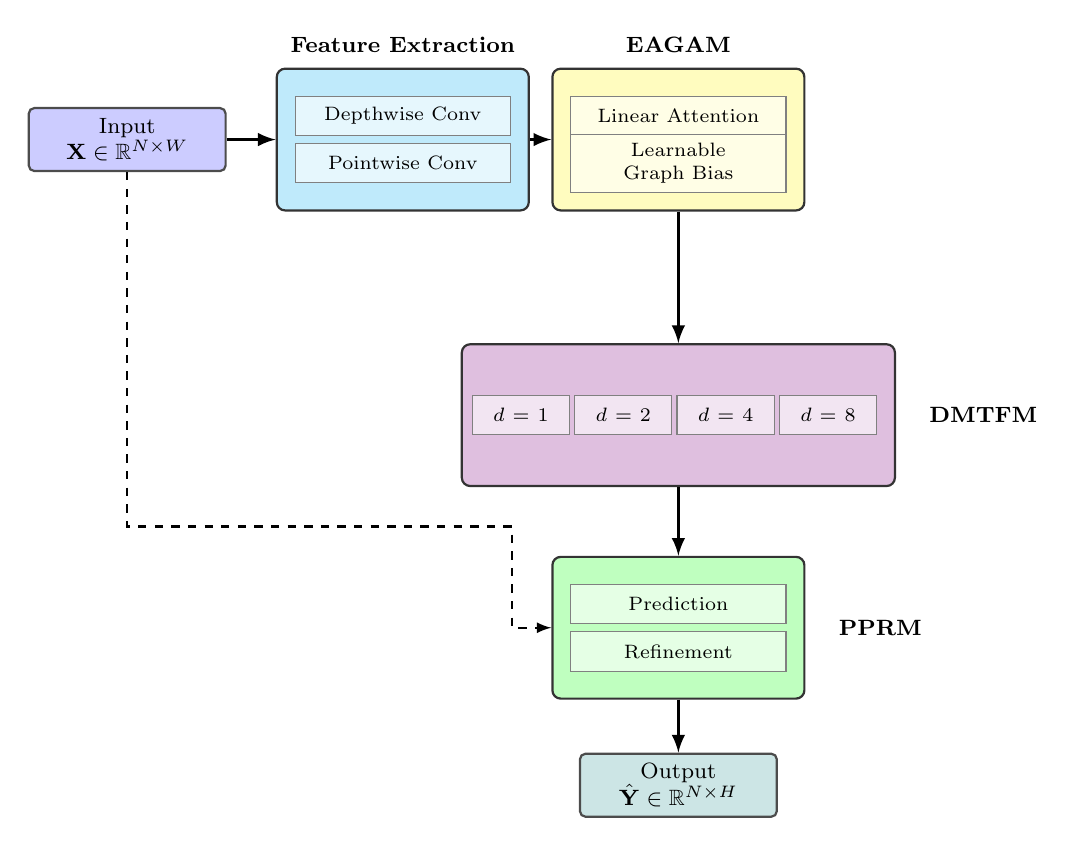
\begin{tikzpicture}[
        font=\footnotesize,
        >=latex,
        node distance = 1.5cm and 2.8cm,
        % Block styles
        module/.style={
            rectangle, 
            draw=black!80, 
            thick,
            rounded corners=3pt,
            minimum height=1.8cm, 
            minimum width=3.2cm,
            align=center,
            fill=#1!25
        },
        submodule/.style={
            rectangle, 
            draw=black!50, 
            minimum height=0.5cm, 
            text width=2.5cm,
            align=center,
            font=\scriptsize,
            fill=#1!10
        },
        data/.style={
            rectangle,
            draw=black!70,
            thick,
            rounded corners=2pt,
            minimum height=0.8cm,
            minimum width=2.5cm,
            align=center,
            fill=#1!20
        },
        arrow/.style={->, thick},
        bigarrow/.style={->, very thick},
        dashedarrow/.style={->, dashed, thick},
        label/.style={font=\footnotesize\bfseries}
    ]
    
    % Input
    \node[data=blue] (input) at (-5, 4) {Input\\$\mathbf{X} \in \mathbb{R}^{N \times W}$};
    
    % Feature Extraction
    \node[module=cyan] (feat) at (-1.5, 4) {};
    \node[label, above=2pt of feat] {Feature Extraction};
    \node[submodule=cyan] (dw) at ([yshift=0.3cm]feat.center) {Depthwise Conv};
    \node[submodule=cyan] (pw) at ([yshift=-0.3cm]feat.center) {Pointwise Conv};
    
    % EAGAM
    \node[module=yellow] (eagam) at (2, 4) {};
    \node[label, above=2pt of eagam] {EAGAM};
    \node[submodule=yellow] (attn) at ([yshift=0.3cm]eagam.center) {Linear Attention};
    \node[submodule=yellow] (bias) at ([yshift=-0.3cm]eagam.center) {Learnable Graph Bias};

    % DMTFM
    \node[module=violet, minimum width=5.5cm] (dmtm) at (2.0, 0.5) {};
    \node[label, above=2pt, right=0.3cm of dmtm] {DMTFM};
    \node[submodule=violet, text width=1.0cm] (s1) at ([xshift=-2.0cm]dmtm.center) {$d=1$};
    \node[submodule=violet, text width=1.0cm] (s2) at ([xshift=-0.7cm]dmtm.center) {$d=2$};
    \node[submodule=violet, text width=1.0cm] (s3) at ([xshift=0.6cm]dmtm.center) {$d=4$};
    \node[submodule=violet, text width=1.0cm] (s4) at ([xshift=1.9cm]dmtm.center) {$d=8$};
    
    % PPRM
    \node[module=green] (ppm) at (2.0, -2.2) {};
    \node[label, above=2pt, right=0.3cm of ppm] {PPRM};
    \node[submodule=green] (pred) at ([yshift=0.3cm]ppm.center) {Prediction};
    \node[submodule=green] (refine) at ([yshift=-0.3cm]ppm.center) {Refinement};
    
    % Output
    \node[data=teal] (output) at (2.0, -4.2) {Output\\$\hat{\mathbf{Y}} \in \mathbb{R}^{N \times H}$};
    
    % Connections
    \draw[bigarrow] (input) -- (feat);
    \draw[bigarrow] (feat) -- (eagam);
    \draw[bigarrow] (eagam) -- (dmtm);
    \draw[bigarrow] (dmtm) -- (ppm);
    \draw[bigarrow] (ppm) -- (output);
    
    \draw[dashedarrow] (input) |- ([yshift=-4.5cm]input.south) -| ([xshift=-0.5cm]ppm.west) -- (ppm);
    
    \end{tikzpicture}
    \caption{Overview of the MSAGAT-Net architecture. The model processes input through four main modules: Feature Extraction using depthwise separable convolutions, EAGAM with linearised attention and learnable graph bias, DMTFM employing multi-scale dilated convolutions (dilation rates $d \in \{1,2,4,8\}$), and PPRM for adaptive forecast refinement. The dashed line represents the skip connection from input to PPRM.}
    \label{fig:msagat_net_architecture}
\end{figure}

\subsection{Feature Extraction}

The first component of the MSAGAT-Net architecture is the feature extraction module, which transforms the raw time-series data into meaningful feature representations whilst maintaining computational efficiency. Given the input time-series data $\mathbf{X} = [\mathbf{x}_{t-w+1}, \mathbf{x}_{t-w+2}, \ldots, \mathbf{x}_t] \in \mathbb{R}^{N \times w}$ for the $N$ regions over a look-back window of $w$ time steps, we need to extract features that capture relevant temporal patterns for each region. This is achieved through a combination of depthwise separable convolutions and low-rank projections, which allow for efficient feature extraction while reducing the risk of overfitting. Depthwise separable convolutions have been shown to significantly reduce the number of parameters and computational complexity while maintaining high performance \cite{chollet2017xception}, and have been successfully applied to spatiotemporal feature extraction \cite{li2023multi, yu2022traffic}. This allows us to efficiently capture the temporal dynamics of epidemic data without incurring the high computational costs associated with traditional convolutional architectures.

\subsubsection{Depthwise Separable Convolutions}

We employ the depthwise separable convolutions to extract temporal features efficiently. This approach significantly reduces the computational complexity and number of parameters whilst maintaining expressive power. The depthwise separable convolution consists of two stages:

For each region's historical window $\mathbf{x}^i_{[t-w+1:t]} \in \mathbb{R}^w$ (the most recent $w$ time steps for region $i$), we first reshape the time-series as a single-channel input. The depthwise convolution applies a separate filter to this channel:

\begin{equation}
\mathbf{z}^i_{\text{depth}} = \text{Conv1D}_{\text{depth}}(\mathbf{x}^i; \boldsymbol{\Theta}_{\text{depth}})
\end{equation}

where $\mathbf{z}^i_{\text{depth}} \in \mathbb{R}^{w \times 1}$ represents the output after depthwise convolution, maintaining the temporal dimension whilst processing each input channel independently.

Following the depthwise convolution, a pointwise convolution (implemented as a 1×1 convolution) is applied to expand the single channel to multiple feature channels:

\begin{equation}
\mathbf{z}^i_{\text{point}} = \text{Conv1D}_{\text{point}}(\mathbf{z}^i_{\text{depth}}; \boldsymbol{\Theta}_{\text{point}})
\end{equation}

where $\mathbf{z}^i_{\text{point}} \in \mathbb{R}^{w \times d_{\text{feat}}}$ represents the features after pointwise convolution, and $d_{\text{feat}} = 16$ is the number of output feature channels.

This decomposition significantly reduces the computational complexity and number of parameters compared to standard convolutions whilst maintaining similar expressive power. Specifically, for a standard convolution with kernel size $k$, input channels $c_{\text{in}}$, and output channels $c_{\text{out}}$, the parameter count is $k \times c_{\text{in}} \times c_{\text{out}}$. In contrast, the depthwise separable convolution requires only $k \times c_{\text{in}} + c_{\text{in}} \times c_{\text{out}}$ parameters.

After each convolutional operation, we apply batch normalisation followed by ReLU activation to enhance training stability and introduce non-linearity:

\begin{equation}
\mathbf{z}^i_{\text{norm}} = \text{ReLU}(\text{BatchNorm}(\mathbf{z}^i_{\text{point}}))
\end{equation}

This normalisation step helps mitigate internal covariate shift during training, whilst the non-linear activation enables the model to capture complex temporal patterns in the epidemic data.

\subsubsection{Low-Rank Feature Projection}

After extracting features using depthwise separable convolutions, we apply a low-rank projection to further reduce dimensionality and capture the most salient features. This projection consists of two linear transformations with a bottleneck in between:

\begin{equation}
\mathbf{F}^i_{\text{low}} = \text{Linear}_{\text{low}}(\text{Flatten}(\mathbf{z}^i_{\text{norm}}))
\end{equation}

\begin{equation}
\mathbf{F}^i = \text{Linear}_{\text{high}}(\mathbf{F}^i_{\text{low}})
\end{equation}

where $\mathbf{F}^i_{\text{low}} \in \mathbb{R}^{d_{\text{bottle}}}$ is the bottleneck representation with dimension $d_{\text{bottle}}$, and $\mathbf{F}^i \in \mathbb{R}^{d_{\text{hidden}}}$ is the final representation of characteristics for region $i$ with dimension $d_{\text{hidden}}$.

The flattening operation converts the convolutional features $\mathbf{z}^i_{\text{norm}} \in \mathbb{R}^{w \times d_{\text{feat}}}$ into a vector of dimension $w \times d_{\text{feat}}$. This is then projected to the bottleneck dimension and subsequently to the hidden dimension.

After applying the low-rank projection to each region's convolutional features, we obtain a comprehensive feature matrix $\mathbf{F} \in \mathbb{R}^{N \times d_{\text{hidden}}}$, where each row $\mathbf{F}^i \in \mathbb{R}^{d_{\text{hidden}}}$ represents the temporal feature embedding for region $i$. This matrix encapsulates the essential temporal dynamics across all $N$ regions in a compact, information-dense representation suitable for subsequent spatial modelling.

The low-rank bottleneck projection ($w \times d_{\text{feat}} \to d_{\text{bottle}} \to d_{\text{hidden}}$) serves multiple critical functions within the architecture. By compressing information through a dimension bottleneck where $d_{\text{bottle}} \ll w \times d_{\text{feat}}$, computational complexity is reduced from $\mathcal{O}(N \times w \times d_{\text{feat}} \times d_{\text{hidden}})$ to $\mathcal{O}(N \times (d_{\text{bottle}} \times d_{\text{hidden}} + w \times d_{\text{feat}} \times d_{\text{bottle}}))$, enabling efficient processing of large-scale spatiotemporal datasets. The bottleneck architecture creates an information constraint that forces the model to distill the most salient temporal patterns, preventing overfitting when training data are limited relative to the high-dimensional input space. Additionally, forcing information through a lower-dimensional manifold encourages separation of relevant signals from noise, allowing subsequent layers to focus on predictive temporal patterns rather than spurious correlations. Finally, the shared projection parameters across all regions create a common latent space that facilitates meaningful comparison and interaction between region features in subsequent graph attention layers.

To stabilise training and enhance feature quality, we apply layer normalisation followed by a non-linear activation:

\begin{equation}
\mathbf{F} = \text{ReLU}(\text{LayerNorm}(\mathbf{F}))
\end{equation}

The layer normalisation operates across the feature dimension, normalising each region's feature vector independently. This addresses internal covariate shift, enabling faster convergence during training whilst making the model robust to variations in feature scale across different regions. The ReLU activation introduces non-linearity essential for modelling complex temporal patterns whilst preserving sparse activation, a property particularly valuable for epidemic time-series that often exhibit punctuated patterns of activity against background stability.

This processed feature matrix $\mathbf{F}$ now encodes the essential temporal characteristics of each region's epidemic time-series in a form optimised for the subsequent EAGAM, which will model dynamic spatial dependencies between regions based on these temporal feature representations. The feature extraction pipeline is illustrated in Figure~\ref{fig:feature_extraction}.

For the Feature Extraction module, we set the feature channel dimension $d_{\text{feat}}$ to 16, the bottleneck dimension $d_{\text{bottle}}$ to 8, and the hidden dimension $d_{\text{hidden}}$ to 32. These values were determined through preliminary experiments to balance the expressiveness of the model with computational efficiency. The convolutional kernel size is set to 3 with appropriate padding to maintain the temporal dimension, thereby capturing local temporal patterns that span 3-5 time steps. This parameter configuration renders the feature extraction module computationally tractable whilst preserving sufficient representational capacity for encoding the diverse temporal dynamics observed in epidemic time-series, a crucial consideration for deployment in resource-constrained epidemic monitoring scenarios.    

\begin{figure}
\centering
\resizebox{1.0\linewidth}{!}{%
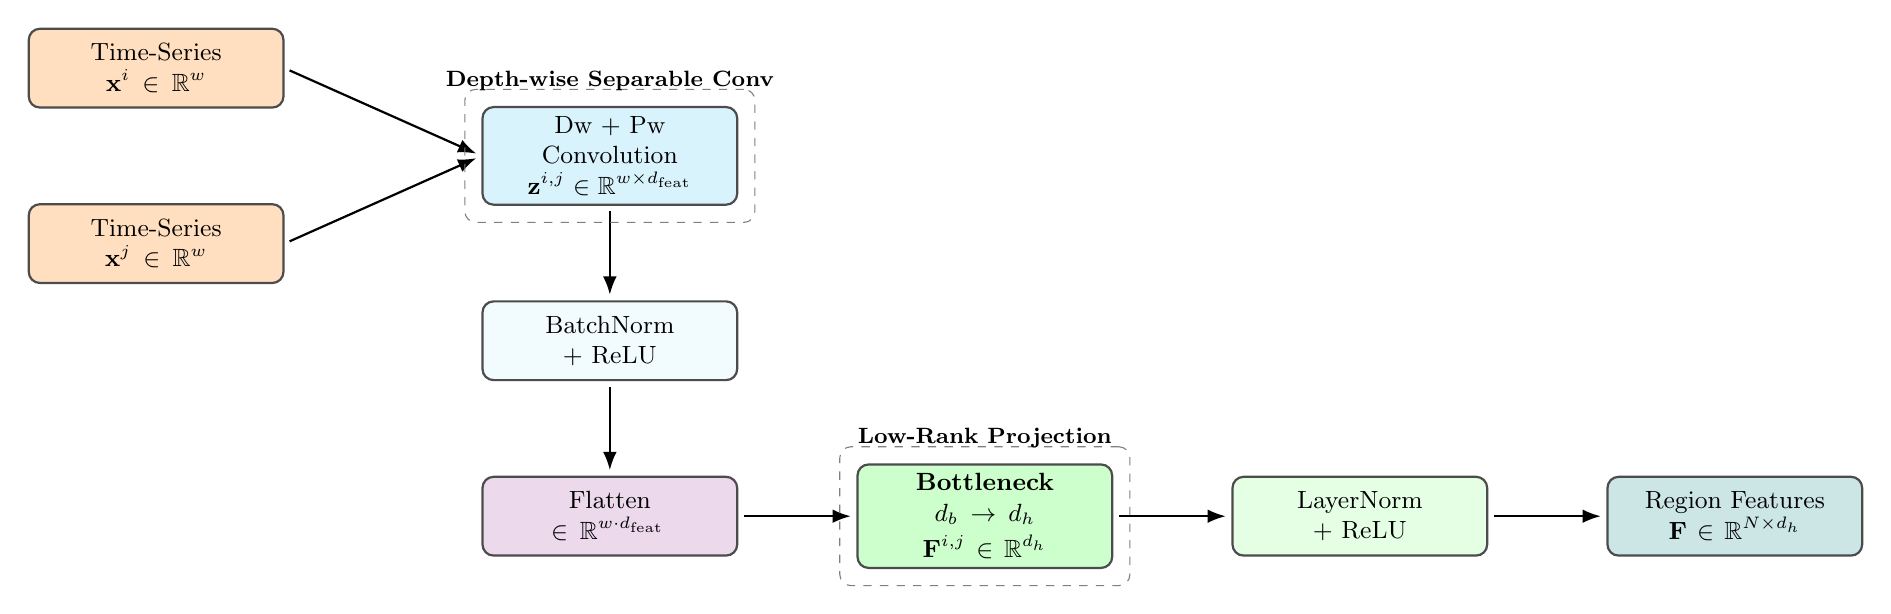
\begin{tikzpicture}[
    font=\small,
    >=Latex,
    block/.style={
        rectangle, draw=black!70, thick,
        rounded corners, align=center,
        minimum height=1cm,  % Increased height
        text width=3cm       % Increased width
    },
    arrow/.style={->, thick, shorten >=2pt, shorten <=2pt},
]
  %––– Inputs (split) –––––––––––––––––––––––––––––––––––––––
  \node (xi) [block, fill=orange!25] {Time‑Series\\$\mathbf{x}^i\!\in\!\mathbb{R}^{w}$};
  \node (xj) [block, fill=orange!25, below=1.2cm of xi] {Time‑Series\\$\mathbf{x}^j\!\in\!\mathbb{R}^{w}$};

  % Compute a point centred between xi and xj for tidy piping
  \path (xi.east) -- (xj.east) coordinate[midway] (midinput);

  %––– Pipeline nodes –––––––––––––––––––––––––––––––––––––––
  \node (sepconv) [block, fill=cyan!15,  right=2.5cm of midinput] {
      Dw + Pw\\Convolution\\
      $\mathbf{z}^{i,j}\!\in\!\mathbb{R}^{w\times d_{\text{feat}}}$};

  \node (bn)   [block, fill=cyan!5, below=1.2cm of sepconv] {BatchNorm\\+ ReLU};

  \node (flat) [block, fill=violet!15, below=1.2cm of bn] {Flatten\\$\!\in\!\mathbb{R}^{w\cdot d_{\text{feat}}}$};

  % Horizontal arrangement for the remaining nodes
  \node (proj) [block, fill=green!20, right=1.5cm of flat] {
      \textbf{Bottleneck}\\$d_b\!\to\! d_h$\\[2pt]
      $\mathbf{F}^{i,j}\!\in\!\mathbb{R}^{d_{h}}$};

  \node (ln) [block, fill=green!10, right=1.5cm of proj] {LayerNorm\\+ ReLU};

  \node (output) [block, fill=teal!20, right=1.5cm of ln] {Region Features\\$\mathbf{F}\!\in\!\mathbb{R}^{N\times d_{h}}$};

  %––– Arrows –––––––––––––––––––––––––––––––––––––––––––––––
  \draw[arrow] (xi.east) -- (sepconv.west);
  \draw[arrow] (xj.east) -- (sepconv.west);
  \draw[arrow] (sepconv.south) -- ++(0,-0.6) -- (bn.north);
  \draw[arrow] (bn.south) -- ++(0,-0.6) -- (flat.north);
  \draw[arrow] (flat.east) -- (proj.west);
  \draw[arrow] (proj.east) -- (ln.west);
  \draw[arrow] (ln.east) -- (output.west);

  %––– Grouping boxes –––––––––––––––––––––––––––––––––––––––
  \usetikzlibrary{fit}
  % \begin{scope}[on background layer] % Removed for IEEEtran compatibility
    \node[draw=black!50, dashed, rounded corners, inner sep=6pt,
          fit=(sepconv)] {};
    \node at (sepconv.north) [above=2pt, font=\footnotesize\bfseries] {Depth‑wise Separable Conv};

    \node[draw=black!50, dashed, rounded corners, inner sep=6pt,
          fit=(proj)] {};
    \node at (proj.north) [above=2pt, font=\footnotesize\bfseries] {Low‑Rank Projection};
  % \end{scope} % Removed for IEEEtran compatibility
\end{tikzpicture}%
}
\caption{Feature‑extraction pipeline. Independent regional time‑series $\mathbf{x}^i$ and $\mathbf{x}^j$ are processed in parallel by depth‑wise and point‑wise convolutions, normalised, flattened, passed through a bottleneck projection ($d_{\text{bottle}}\!\to\! d_{\text{hidden}}$), and normalised again to yield region‑level feature vectors $\mathbf F$.}
\label{fig:feature_extraction}
\end{figure}

\subsection{Efficient Adaptive Graph Attention with Low-Rank Decomposition}

The second core component of our MSAGAT-Net architecture is EAGAM. Traditional approaches to spatial modelling often rely on fixed adjacency matrices based on geographical proximity or administrative boundaries, which do not capture the evolving nature of epidemic spread influenced by factors such as population mobility, healthcare referral patterns, and socioeconomic connections. Based on the principles of graph attention networks \cite{velickovic2017graph}, our EAGAM adaptively learns the relationships between regions based on their feature representations, rather than being constrained by a predefined graph structure. This adaptive approach allows the model to discover and leverage spatial dependencies that may not be immediately apparent from geographical proximity alone, and to adjust these dependencies as the epidemic evolves.

A significant challenge in implementing graph attention mechanisms for large-scale epidemic forecasting problems is computational complexity. Standard softmax-based attention mechanisms in graph neural networks (GNNs) typically incur quadratic $\mathcal{O}(N^2)$ complexity with respect to the number of nodes, making them prohibitively expensive for large graphs. Additionally, these methods often suffer from over-smoothing when modelling long-range dependencies, where node representations become increasingly similar after multiple message-passing iterations.

Recent advances in efficient attention mechanisms have shown that low-rank decomposition techniques can substantially reduce computational complexity whilst maintaining expressive power. Several influential works have explored this direction. Researchers such as \cite{puny2020global} propose a low-rank global attention (LRGA), an adaptive module that replaces the total attention of the dot product in GNN with a decomposed low-rank form. \cite{kong2023low} present the Global Representation Key (GRK) attention layer, where the attention scores of each node are calculated using a shared projection of the features of its neighbours. A learnt adaptive low-rank matrix captures the most salient structural information, mitigating over-smoothing and improving performance on graphs. While \cite{yang2023self} embeds an adaptive low-rank decomposition step in each propagation layer within each ego network to concentrate the message passing on the most prominent low-dimensional subspaces. This lets the model adaptively focus on the most informative subspace per node, improving robustness without labels. These studies collectively demonstrate that low-rank factorisation offers an efficient, scalable, and expressive alternative to full-rank attention in graph architectures, motivating the design of this module in our framework.

Motivated by these advances, EAGAM employs a linearised attention mechanism that combines low‑rank decomposition with a novel graph bias message passing mechanism. Rather than computing the full attention matrix between all pairs of regions (which incurs $\mathcal{O}(N^2)$ complexity for traditional softmax attention), we use a linearised formulation that reduces complexity to $\mathcal{O}(N)$ through fixed-rank bottleneck projections (bottleneck dimension $d_b = 8$), scaling linearly with the number of regions. Efficiency arises from (i) low‑rank bottleneck projections for query, key, and value representations, and (ii) a linearised attention computation that avoids explicit construction of the $N\times N$ attention matrix whilst maintaining the capacity to learn complex spatial dependencies. A key innovation of our approach is the integration of a learnable graph bias directly into the forward computation through normalised low-rank message passing, rather than using it solely for regularisation as in prior work. This enables the model to leverage persistent spatial relationships during inference whilst maintaining linear complexity. The EAGAM module comprises six components: (1) bottleneck projections for QKV, (2) multi‑head attention with ELU‑based linearisation, (3) normalisation for numerical stability, (4) learnable graph structure bias, (5) graph bias message passing for forward integration, and (6) attention regularisation to promote sparsity.


\subsubsection{Bottleneck Projection}

Given the feature matrix $\mathbf{F} \in \mathbb{R}^{N \times d_{\text{hidden}}}$ from the feature extraction module, where $N$ is the number of regions and $d_{\text{hidden}}$ is the hidden dimension, we first project these features into query, key, and value representations through an efficient bottleneck projection:

\begin{equation}
\mathbf{Q}_{\text{low}}, \mathbf{K}_{\text{low}}, \mathbf{V}_{\text{low}} = \text{Split}(\text{Linear}_{\text{low}}(\mathbf{F}), 3)
\end{equation}

where $\text{Linear}_{\text{low}}: \mathbb{R}^{d_{\text{hidden}}} \rightarrow \mathbb{R}^{3 \times d_{\text{bottle}}}$ projects the features into a lower-dimensional space and $\text{Split}$ divides the output into three separate tensors of dimension $\mathbb{R}^{N \times d_{\text{bottle}}}$.

These low-dimensional projections are then expanded back to the full hidden dimension:

\begin{equation}
\mathbf{Q}, \mathbf{K}, \mathbf{V} = \text{Split}(\text{Linear}_{\text{high}}([\mathbf{Q}_{\text{low}}; \mathbf{K}_{\text{low}}; \mathbf{V}_{\text{low}}]), 3)
\end{equation}

where $\text{Linear}_{\text{high}}: \mathbb{R}^{3 \times d_{\text{bottle}}} \rightarrow \mathbb{R}^{3 \times d_{\text{hidden}}}$ and each of $\mathbf{Q}, \mathbf{K}, \mathbf{V} \in \mathbb{R}^{N \times d_{\text{hidden}}}$.

This bottleneck projection significantly reduces the parameter count from $\mathcal{O}(3 \times d_{\text{hidden}}^2)$ to $\mathcal{O}(3 \times d_{\text{hidden}} \times d_{\text{bottle}})$, where $d_{\text{bottle}} \ll d_{\text{hidden}}$.

\subsubsection{Multi-Head Attention Mechanism}

To enhance the model's capacity to capture different types of inter-regional relationships, we implement a multi-head attention mechanism where the hidden representations are split into $h$ heads, each with dimension $d_{\text{head}} = d_{\text{hidden}} / h$:

\begin{equation}
\mathbf{Q}^{(i)}, \mathbf{K}^{(i)}, \mathbf{V}^{(i)} \in \mathbb{R}^{N \times d_{\text{head}}}, \quad i \in \{1, 2, \ldots, h\}
\end{equation}

For efficient computation, we reshape these tensors to explicitly represent the multiple heads:

\begin{equation}
\mathbf{Q}_h = \text{Reshape}(\mathbf{Q}, [N, h, d_{\text{head}}])
\end{equation}
\begin{equation}
\mathbf{K}_h = \text{Reshape}(\mathbf{K}, [N, h, d_{\text{head}}])
\end{equation}
\begin{equation}
\mathbf{V}_h = \text{Reshape}(\mathbf{V}, [N, h, d_{\text{head}}])
\end{equation}

We then transpose the first two dimensions to facilitate batch-wise processing across attention heads:

\begin{align}
\mathbf{Q}_h &= \text{Transpose}(\mathbf{Q}_h, 0, 1) \\
\mathbf{K}_h &= \text{Transpose}(\mathbf{K}_h, 0, 1) \\
\mathbf{V}_h &= \text{Transpose}(\mathbf{V}_h, 0, 1)
\end{align}

resulting in tensors of shape $[h, N, d_{\text{head}}]$.

A key innovation in our approach is the specific attention computation mechanism employed within each head. Rather than relying on standard scaled dot-product attention with softmax, we employ an enhanced mechanism with better numerical stability and more nuanced relationship modelling.

First, we apply the Exponential Linear Unit (ELU) activation function followed by adding a constant value of 1 to both query and key representations:

\begin{equation}
\hat{\mathbf{Q}}_h = \text{ELU}(\mathbf{Q}_h) + 1
\end{equation}
\begin{equation}
\hat{\mathbf{K}}_h = \text{ELU}(\mathbf{K}_h) + 1
\end{equation}

This transformation, known as the ELU+1 kernel trick \cite{katharopoulos2020transformers}, ensures that all attention inputs are strictly positive, which is essential for the linearisation that follows. The key insight is that standard softmax attention computes $\text{softmax}(\mathbf{Q}\mathbf{K}^T)\mathbf{V}$, requiring explicit construction of the $N \times N$ attention matrix with $\mathcal{O}(N^2)$ complexity. By using a positive feature map $\phi(\cdot) = \text{ELU}(\cdot) + 1$, we can exploit the associativity of matrix multiplication: instead of computing $(\phi(\mathbf{Q})\phi(\mathbf{K})^T)\mathbf{V}$, we compute $\phi(\mathbf{Q})(\phi(\mathbf{K})^T\mathbf{V})$, reducing complexity to $\mathcal{O}(N \cdot d_{\text{head}}^2)$---linear in the number of regions.

Next, we compute the key-value product for each attention head:

\begin{equation}
\mathbf{KV}_h = \hat{\mathbf{K}}_h^T \mathbf{V}_h
\end{equation}

where $\mathbf{KV}_h \in \mathbb{R}^{h \times d_{\text{head}} \times d_{\text{head}}}$. This operation captures the relationships between keys and values, allowing the model to learn how to weight the features of different regions based on their similarity.

To ensure stable normalisation, we calculate a normalisation factor based on the sum of keys:

\begin{equation}
\mathbf{z} = \frac{1}{\sum_{d=1}^{d_{\text{head}}} \hat{\mathbf{K}}_h + \epsilon}
\end{equation}

where the sum is taken over the feature dimension $d_{\text{head}}$ for each node in each head, $\epsilon = 10^{-8}$ prevents division by zero, and $\mathbf{z} \in \mathbb{R}^{h \times N}$ represents the normalisation factor for each node in each attention head. This operation ensures stable normalisation across the attention heads, allowing for effective learning of inter-regional relationships. 

The final linear attention output for each head is computed as:

\begin{equation}
\mathbf{O}_{\text{linear}} = (\hat{\mathbf{Q}}_h \mathbf{KV}_h) \odot \mathbf{z}
\end{equation}

where $\mathbf{O}_{\text{linear}} \in \mathbb{R}^{h \times N \times d_{\text{head}}}$ represents the attended features across all heads, and $\odot$ denotes element-wise multiplication with broadcasting of the normalisation factor $\mathbf{z}$ across the feature dimension.

\subsubsection{Learnable Graph Structure}

An important feature of our EAGAM is the incorporation of a learnable graph structure bias. Unlike traditional graph attention networks that rely solely on node features for computing attention, we include a learnable bias term that captures persistent structural relationships between regions that may not be evident from the node features alone.

This bias is implemented as a low-rank decomposition for parameter efficiency:

\begin{equation}
\mathbf{B} = \mathbf{U} \mathbf{V}
\end{equation}

where $\mathbf{U} \in \mathbb{R}^{h \times N \times d_{\text{bias}}}$ and $\mathbf{V} \in \mathbb{R}^{h \times d_{\text{bias}} \times N}$ are learnable parameters and $d_{\text{bias}} \ll N$ is the bottleneck dimension of the bias term (set equal to $d_{\text{bottle}} = 8$ in our implementation). Both $\mathbf{U}$ and $\mathbf{V}$ are initialised using Xavier uniform initialisation \cite{glorot2010understanding} to ensure balanced gradient flow across heads and maintain stable training dynamics from the outset. This learnable bias $\mathbf{B} \in \mathbb{R}^{h \times N \times N}$ provides an innovative mechanism for the model to learn persistent spatial structures that complement data-driven attention patterns.

\subsubsection{Graph Bias Message Passing}

Rather than using the graph bias solely for regularisation, we integrate it directly into the forward computation through a normalised low-rank message passing operation. This approach maintains $\mathcal{O}(N)$ complexity by exploiting the low-rank factorisation $\mathbf{B} = \mathbf{U}\mathbf{V}$ to avoid materialising the full $N \times N$ bias matrix.

To ensure stable message passing with non-negative weights, we first apply a positivity transformation to the low-rank factors:

\begin{equation}
\hat{\mathbf{U}} = \text{ELU}(\mathbf{U}) + 1, \quad \hat{\mathbf{V}} = \text{ELU}(\mathbf{V}) + 1
\end{equation}

The graph bias message passing output is then computed as:

\begin{equation}
\mathbf{O}_{\text{bias}} = \frac{\hat{\mathbf{U}} (\hat{\mathbf{V}} \mathbf{V}_h)}{\hat{\mathbf{U}} (\hat{\mathbf{V}} \mathbf{1}) + \epsilon}
\end{equation}

where $\mathbf{V}_h$ represents the value representations, $\mathbf{1}$ is a vector of ones, and $\epsilon = 10^{-8}$ prevents division by zero. The numerator computes $\hat{\mathbf{U}} (\hat{\mathbf{V}} \mathbf{V}_h) \in \mathbb{R}^{h \times N \times d_{\text{head}}}$ through two sequential matrix multiplications, each with complexity $\mathcal{O}(N \cdot d_{\text{bias}} \cdot d_{\text{head}})$. The denominator provides row-wise normalisation analogous to the normalisation in standard attention mechanisms.

This message passing output is combined with the linear attention output:

\begin{equation}
\mathbf{O}_h = \mathbf{O}_{\text{linear}} + \text{Dropout}(\mathbf{O}_{\text{bias}})
\end{equation}

By integrating the learned graph structure directly into the forward pass, the model can leverage persistent spatial relationships during inference whilst maintaining the computational efficiency of linearised attention.

\subsubsection{Optional Adjacency Prior Integration}

Unlike state-of-the-art baselines that \emph{require} predefined adjacency matrices, MSAGAT-Net learns spatial relationships entirely from data. However, when prior knowledge about regional connectivity is available (e.g., geographical proximity or mobility patterns), it can be optionally incorporated to accelerate learning and improve performance. This is achieved through a learnable gating mechanism that combines the learned graph structure with the provided adjacency prior:

\begin{equation}
\mathbf{O}_{\text{bias}}' = (1 - \sigma(g)) \cdot \mathbf{O}_{\text{bias}} + \sigma(g) \cdot \tilde{\mathbf{A}} \mathbf{V}_h
\end{equation}

where $g$ is a learnable gate parameter initialised to a small value (e.g., 0.1), $\sigma(\cdot)$ denotes the sigmoid function ensuring the gate remains in $[0, 1]$, and $\tilde{\mathbf{A}}$ is the symmetrically normalised adjacency matrix with added self-loops:

\begin{equation}
\tilde{\mathbf{A}} = \mathbf{D}^{-1/2}(\mathbf{A} + \mathbf{I})\mathbf{D}^{-1/2}
\end{equation}

where $\mathbf{D}$ is the degree matrix and $\mathbf{I}$ is the identity matrix. This formulation has several desirable properties:

\begin{itemize}
    \item \textbf{Flexibility:} When no adjacency is provided, the model operates using only the learned graph bias, matching the default behaviour.
    \item \textbf{Adaptability:} The gate parameter $g$ is learned during training, allowing the model to determine the optimal balance between prior knowledge and data-driven patterns.
    \item \textbf{Efficiency:} The adjacency-based message passing $\tilde{\mathbf{A}} \mathbf{V}_h$ has $\mathcal{O}(|E|)$ complexity where $|E|$ is the number of edges, typically sparse for geographical adjacency.
\end{itemize}

This design choice distinguishes MSAGAT-Net from existing approaches: baselines such as EpiGNN, Cola-GNN, and DCRNN mandate adjacency matrices as required input, whereas MSAGAT-Net can function without them whilst optionally benefiting from prior knowledge when available. Importantly, our experimental analysis (Section~\ref{sec:results}) demonstrates that learning spatial relationships from data actually \emph{outperforms} using predefined geographical adjacency, validating the fundamental premise of our approach.

\subsubsection{Attention Regularisation}

To promote sparse and interpretable spatial relationships, we apply L1 regularisation to the graph structure bias:

\begin{equation}
\mathcal{L}_{\text{attn}} = \lambda \|\mathbf{B}\|_1
\end{equation}

where $\lambda$ is the learnable regularisation weight. This regularisation encourages the model to learn sparse, interpretable spatial dependency patterns in the graph bias whilst maintaining the computational efficiency of linearised attention. The value of $\lambda$ is initialised to $10^{-5}$ and adapted during training through gradient descent in log-domain (ensuring positivity), allowing the model to automatically balance forecast accuracy with attention sparsity.

After computing the attended values for each head, we combine them and project back to the original feature dimension:

\begin{equation}
\mathbf{O} = \text{Reshape}(\text{Transpose}(\mathbf{O}_h, 0, 1), [N, d_{\text{hidden}}])
\end{equation}

Similarly to the input projection, we employ a low-rank output projection for efficiency:

\begin{equation}
\mathbf{O}_{\text{low}} = \text{Linear}_{\text{out\_low}}(\mathbf{O})
\end{equation}

\begin{equation}
\mathbf{O}_{\text{final}} = \text{Linear}_{\text{out\_high}}(\mathbf{O}_{\text{low}})
\end{equation}

where $\mathbf{O}_{\text{low}} \in \mathbb{R}^{N \times d_{\text{bottle}}}$ and $\mathbf{O}_{\text{final}} \in \mathbb{R}^{N \times d_{\text{hidden}}}$.

The output of EAGAM, $\mathbf{O}_{\text{final}}$, represents the features of the region after incorporating spatial dependencies. This output, along with the attention regularisation loss $\mathcal{L}_{\text{attn}}$, is passed to the subsequent DMTFM for further processing.

For the EAGAM module, we set the number of attention heads to $h=4$ and the bottleneck dimension to $d_{\text{bottle}}=8$. These values were determined through preliminary experiments to provide an optimal balance between capturing diverse spatial dependency patterns and the maintenance of computational efficiency through low-rank decomposition. The attention regularisation weight $\lambda$ is set to $10^{-5}$, which was empirically found to promote sparse, interpretable attention patterns without overly constraining the model's capacity to learn complex spatial relationships. This configuration allows EAGAM to model dynamic spatial dependencies efficiently whilst avoiding the computational overhead of full-rank attention mechanisms. Figure~\ref{fig:eagam_module} presents the data flow through the EAGAM module. 

\begin{figure}
\centering
%–— 1. We still fix the width to \linewidth; the height now shrinks naturally –—
\resizebox{\linewidth}{!}{%
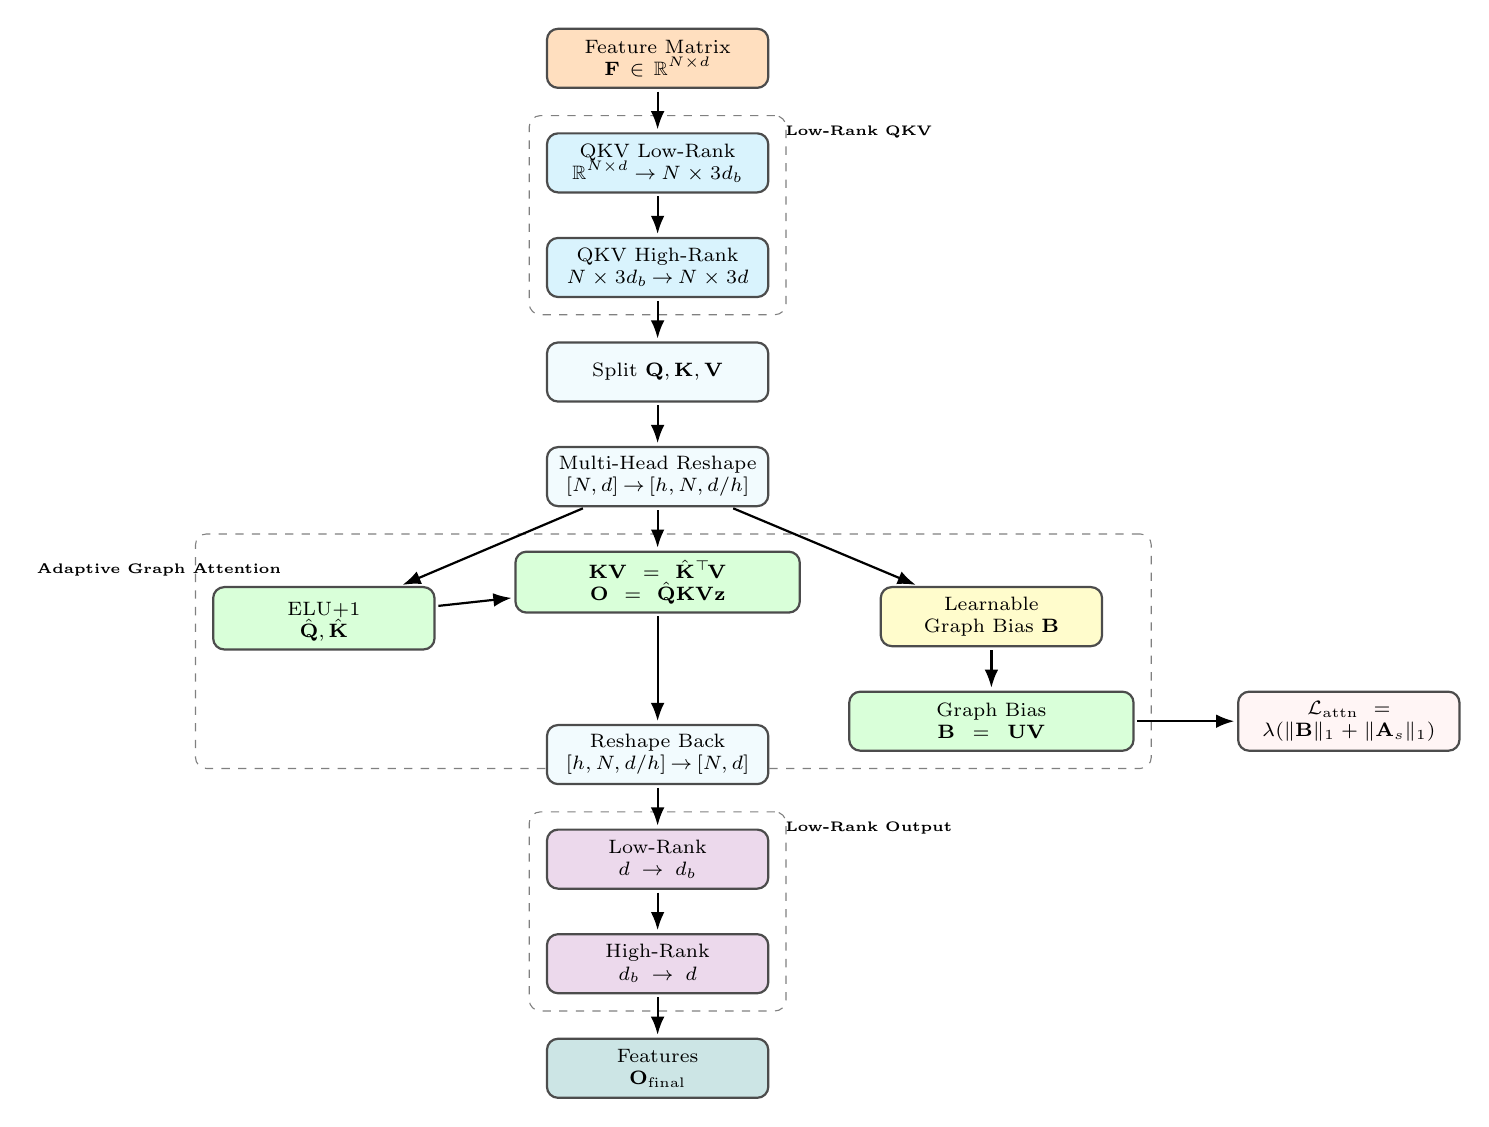
\begin{tikzpicture}[
    %–––– GLOBAL STYLE TWEAKS ––––
    font=\scriptsize,                                % smaller text
    >=Latex,
    node distance = 0.55cm and 1.6cm,                % default vert / horiz gap
    block/.style = {rectangle, draw=black!70, thick,
                    rounded corners, align=center,
                    minimum height=0.75cm,           % lower boxes
                    text width=2.6cm,                % narrower boxes
                    inner sep=3pt},                  % tighter padding
    wideblock/.style = {block, text width=3.4cm},    % a bit wider
    arrow/.style = {->, thick, shorten >=1pt, shorten <=1pt},
]
%–––– MAIN FLOW ––––
\node (input)      [block, fill=orange!25] {Feature Matrix\\$\mathbf{F}\!\in\!\mathbb{R}^{N\times d}$};

\node (qkv_low)    [block,  fill=cyan!15,  below=of input]          {QKV Low‑Rank\\$\mathbb{R}^{N\times d}\!\to\! N\times3d_b$};

\node (qkv_high)   [block,  fill=cyan!15,  below=of qkv_low]        {QKV High‑Rank\\$N\times3d_b\!\to\! N\times3d$};

\node (split)      [block,  fill=cyan!5,   below=of qkv_high]       {Split $\mathbf Q,\mathbf K,\mathbf V$};

\node (reshape)    [block,  fill=cyan!5,   below=of split]          {Multi‑Head Reshape\\$[N,d]\!\to\![h,N,d/h]$};

%–––– PARALLEL BRANCH (three nodes at same depth) ––––
\node (qk_proc)    [block,  fill=green!15, below left=1.0cm and 1.4cm of reshape] {\rule{0pt}{0.9em}ELU$+1$\\$\hat{\mathbf Q},\hat{\mathbf K}$};

\node (graph_bias) [block,  fill=yellow!20, below right=1.0cm and 1.4cm of reshape] {Learnable\\Graph Bias $\mathbf B$};

\node (attn_comp)  [wideblock, fill=green!15, below=of reshape]     {$\mathbf{KV}=\hat{\mathbf K}^\top\!\mathbf V$\\
                                                                     $\mathbf O=\hat{\mathbf Q}\mathbf{KV}\mathbf z$};

%–––– ATTENTION SCORE / REG ––––
\node (attn_scores)[wideblock, fill=green!15, below=of graph_bias]  {Graph Bias\\$\mathbf B=\mathbf{UV}$};

\node (attn_reg)   [block,      fill=pink!15,  right=1.3cm of attn_scores] {$\mathcal L_{\text{attn}}=\lambda(\|\mathbf B\|_1+\|\mathbf A_s\|_1)$};

%–––– OUTPUT PATH ––––
\node (reshape_out) [block, fill=cyan!5,   below=1.4cm of attn_comp] {Reshape Back\\$[h,N,d/h]\!\to\![N,d]$};

\node (out_low)     [block, fill=violet!15, below=of reshape_out]   {Low‑Rank\\$d\!\to\! d_b$};

\node (out_high)    [block, fill=violet!15, below=of out_low]       {High‑Rank\\$d_b\!\to\! d$};

\node (output)      [block, fill=teal!20,   below=of out_high]      {Features\\$\mathbf O_{\text{final}}$};

%–––– ARROWS ––––
\foreach \a/\b in {
  input/qkv_low, qkv_low/qkv_high, qkv_high/split, split/reshape,
  reshape/qk_proc,  reshape/attn_comp, reshape/graph_bias,
  qk_proc/attn_comp, graph_bias/attn_scores,
  attn_scores/attn_reg, attn_comp/reshape_out,
  reshape_out/out_low, out_low/out_high, out_high/output}
  \draw[arrow] (\a) -- (\b);

%–––– GROUP BOXES (dashed) ––––
\usetikzlibrary{fit}
\begin{scope}[on background layer]
  \node [draw=black!50, dashed, rounded corners, inner sep=6pt,
         fit=(qkv_low)(qkv_high)] {};
  \node at (qkv_low.north) [above=1pt, right=0pt and 1.5cm, font=\tiny\bfseries] {Low‑Rank QKV};

  \node [draw=black!50, dashed, rounded corners, inner sep=6pt,
         fit=(qk_proc)(attn_comp)(graph_bias)(attn_scores)] {};
  \node at (qk_proc.north west) [above left=0pt and -1.0cm, font=\tiny\bfseries] {Adaptive Graph Attention};

  \node [draw=black!50, dashed, rounded corners, inner sep=6pt,
         fit=(out_low)(out_high)] {};
  \node at (out_low.north) [above=1pt, right=0pt and 1.5cm, font=\tiny\bfseries] {Low‑Rank Output};
\end{scope}
\end{tikzpicture}}%
% \caption{Flow of data and structure in the EAGAM module.}
\caption{Data flow in the EAGAM module. Input features undergo low-rank QKV projections, followed by linearised attention computation with learnable graph bias for spatial dependency modelling, and low-rank output projection.}
\label{fig:eagam_module}
\end{figure}

Figure \ref{fig:eagam_module} illustrates the flow of data through the EAGAM module. The input feature matrix $\mathbf{F}$ is processed through low-rank projections to obtain query, key, and value representations. These representations are then reshaped for multi-head attention computation, where the adaptive graph attention mechanism is applied. The learnable graph structure bias is incorporated into the attention scores, and L1 regularisation is applied to promote sparse attention patterns. Finally, the output features are obtained through high-rank projections, ready for further processing in DMTFM.

\subsection{Dilated Multi-Scale Temporal Feature Module}

The third major component of the proposed MSAGAT-Net architecture is the Dilated Multi-Scale Temporal Feature Module (DMTFM), which addresses a fundamental challenge in epidemic forecasting: modelling temporal dependencies across multiple time scales. Epidemics exhibit complex temporal dynamics that span various scales, including short-term fluctuations (e.g., reporting delays or weekend effects), medium-term patterns (e.g., incubation or transmission cycles), and long-term trends (e.g., seasonal variations or behavioural changes) \cite{Stone2007Seasonal, Panja2022Epicasting, Qiu2024MSGNN}. Accurate forecasting therefore requires models capable of effectively capturing these multi-scale temporal dynamics.


Deng et al. \cite{dengColaGNNCrosslocationAttention2020a} introduce the idea of multi-scale dilated convolutional with the same filter and stride sides but different dilation rates, which Xie et al. \cite{xie2022epignn} improved by making use of the multi-scale convolution to capture features. Building on this, the DMTFM employs parallel dilated convolutional layers to efficiently capture temporal dependencies across multiple scales using the output from the EAGAM. This approach enables the model to maintain an awareness of both immediate and distant temporal relationships whilst controlling parameter count and computational complexity.


\subsubsection{Dilated Convolutions for Multi-scale Processing}

The core of our DMTFM is a set of parallel convolutional branches operating at different dilation rates. For a given input feature tensor $\mathbf{G} \in \mathbb{R}^{B \times N \times d_{\text{hidden}}}$ (where $B$ is the batch size, $N$ is the number of regions, and $d_{\text{hidden}}$ is the hidden dimension), we first transpose the tensor to prepare for 1D convolutions along the temporal dimension:

\begin{equation}
\mathbf{G}_{\text{conv}} = \text{Transpose}(\mathbf{G}, 1, 2)
\end{equation}

resulting in a tensor of shape $[B, d_{\text{hidden}}, N]$. We then process this tensor through $S$ parallel branches, each consisting of a dilated convolutional layer with a specific dilation rate, followed by batch normalisation, ReLU activation and dropout:

\begin{equation}
\mathbf{H}^{(i)} = \text{Dropout}(\text{ReLU}(\text{BatchNorm}(\text{Conv1D}(\mathbf{G}_{\text{conv}}; k, d^{(i)}))))
\end{equation}

We employ batch normalisation rather than layer normalisation in DMTFM for two principal reasons. First, convolutional layers benefit from batch normalisation's channel-wise statistics, which stabilise feature distributions across the hidden dimension whilst preserving temporal structure within each channel. Second, batch normalisation provides implicit regularisation through mini-batch statistics, complementing the explicit dropout regularisation and helping prevent overfitting on the often noisy epidemic time-series data.

where $i \in \{1, 2, \ldots, S\}$ indexes the scale, $k$ is the kernel size (set to 3 by default), and $d^{(i)} = 2^{i-1}$ is the dilation rate for the scale $i$. Each branch produces an output tensor $\mathbf{H}^{(i)} \in \mathbb{R}^{B \times d_{\text{hidden}} \times N}$.

The increasing dilation rates create an exponentially expanding receptive field across the branches. For a single dilated convolutional layer with kernel size $k$ and dilation rate $d$, the receptive field is given by:

\begin{equation}
\text{RF} = k + (k - 1) \times (d - 1) = 1 + (k - 1) \times d
\end{equation}

With our configuration of $k = 3$, this yields receptive fields of 3, 5, 9, and 17 time steps for scales 1, 2, 3, and 4 respectively. Scale 1 ($d^{(1)} = 1$) captures immediate temporal dependencies spanning 3 time steps, scale 2 ($d^{(2)} = 2$) captures medium-range dependencies spanning 5 time steps (approximately one week at daily resolution), scale 3 ($d^{(3)} = 4$) captures longer-range dependencies spanning 9 time steps (over one week), and scale 4 ($d^{(4)} = 8$) captures extended patterns spanning 17 time steps (over two weeks), enabling the model to capture weekly and bi-weekly periodicity common in epidemic reporting patterns.

This multi-scale approach allows the model to efficiently capture a wide range of temporal dependencies without requiring deep sequential processing, which is particularly advantageous for epidemic time-series that often exhibit both rapid changes and gradual trends.

\subsubsection{Adaptive Scale Fusion}

Rather than simply concatenating or averaging the outputs from different scales, we implement an adaptive fusion mechanism that allows the model to learn the relative importance of each temporal scale. This is achieved through learnable fusion weights:

\begin{equation}
\boldsymbol{\alpha} = \text{softmax}(\mathbf{w})
\end{equation}

where $\mathbf{w} \in \mathbb{R}^S$ is a vector of learnable parameters and $\boldsymbol{\alpha} \in \mathbb{R}^S$ represents the normalised importance weights for each scale.

The multi-scale features are then fused using these weights:

\begin{equation}
\mathbf{H}_{\text{fused}} = \sum_{i=1}^{S} \alpha_i \mathbf{H}^{(i)}
\end{equation}

where $\mathbf{H}_{\text{fused}} \in \mathbb{R}^{B \times d_{\text{hidden}} \times N}$ is the scale-fused feature representation.



\begin{figure}
\centering
\includegraphics[width=0.7\textwidth]{figs/DMTFM.png}
% \caption{Flow of data in the MTFM architecture.}
\caption{Data flow in the MTFM module. Spatial features from AGAM are processed through four parallel dilated convolutional branches (dilation rates 1, 2, 4, 8), adaptively fused using learnable weights, and combined with residual connections.}
\label{fig:mtfm_module}
\end{figure}


\subsubsection{Bottleneck Projection and Residual Connection}

To enhance training stability and allow for more effective feature transformation, we apply a low-rank bottleneck projection to the fused features:

\begin{equation}
\mathbf{H}_{\text{low}} = \text{Linear}_{\text{fusion\_low}}(\text{Transpose}(\mathbf{H}_{\text{fused}}, 1, 2))
\end{equation}

\begin{equation}
\mathbf{H}_{\text{proj}} = \text{Linear}_{\text{fusion\_high}}(\mathbf{H}_{\text{low}})
\end{equation}

where $\mathbf{H}_{\text{low}} \in \mathbb{R}^{B \times N \times d_{\text{bottle}}}$ is the bottleneck representation with dimension $d_{\text{bottle}} \ll d_{\text{hidden}}$, and $\mathbf{H}_{\text{proj}} \in \mathbb{R}^{B \times N \times d_{\text{hidden}}}$ is the projected representation.

We then apply layer normalisation and a residual connection to facilitate gradient flow during training:

\begin{equation}
\mathbf{H}_{\text{final}} = \text{LayerNorm}(\text{Transpose}(\mathbf{H}_{\text{fused}}, 1, 2) + \mathbf{H}_{\text{proj}})
\end{equation}

where $\mathbf{H}_{\text{final}} \in \mathbb{R}^{B \times N \times d_{\text{hidden}}}$ is the final output of the DMTFM.

For the DMTFM module, we set the number of temporal scales to $S=4$ with exponentially increasing dilation rates of $\{1, 2, 4, 8\}$ and a convolutional kernel size of $k=3$. This multi-scale configuration enables the module to capture temporal dependencies at multiple granularities, ranging from immediate neighbour relationships (1-step) to medium-range patterns (3-5 time steps), weekly-scale patterns (7-11 time steps), and bi-weekly patterns (15-17 time steps). These scales are particularly well suited to epidemic dynamics, where transmission patterns manifest across multiple temporal horizons. The hidden dimension $d_{\text{hidden}}$ is preserved throughout the module to maintain information capacity, whilst the bottleneck dimension for the fusion projection is set to $d_{\text{bottle}} = 8$ to reduce parameters. To mitigate overfitting on the noisy and often irregular epidemic time-series, we apply dropout with probability 0.2 after each convolutional layer to regularise the model. This dropout rate was determined through preliminary hyperparameter tuning to effectively balance model expressiveness with robustness to noise patterns characteristic of real-world epidemic surveillance data. Figure~\ref{fig:dmtfm_module} presents a detailed representation of this module's architecture. 


\subsection{Progressive Multi-Horizon Forecast Refinement}

The final component of our MSAGAT-Net architecture is the Progressive Refinement Multi-Horizon Forecast Module (PPRM), which generates accurate forecasts across multiple future time steps. Multi-horizon forecasting presents a significant challenge in epidemiological prediction: whilst the preceding modules extract spatiotemporal features, converting these features into reliable forecasts requires addressing how forecast errors can compound over extended horizons.

The existing literature demonstrates that forecast errors accumulate with increasing forecast horizons \cite{BENTAIEB20127067, chandra2021evaluation}, making direct multistep prediction particularly challenging. The PPRM addresses this by incorporating an adaptive refinement mechanism that balances model-based forecasts with trend-based extrapolations. This design draws on concepts from adaptive gating mechanisms in recurrent neural networks \cite{hochreiter1997long} and is motivated by the observation that the recent epidemic trajectory provides valuable information for near-term forecasting.


\subsubsection{Low-Rank Forecast Projection}

Given the spatiotemporal feature tensor $\mathbf{H}_{\text{final}} \in \mathbb{R}^{B \times N \times d_{\text{hidden}}}$ from the multi-scale Fusion Module, where $B$ is the batch size, $N$ is the number of regions, and $d_{\text{hidden}}$ is the hidden dimension, we first apply a bottleneck projection to distil the most forecast-relevant information:

\begin{equation}
\mathbf{P}_{\text{low}} = \text{Linear}_{\text{pred\_low}}(\mathbf{H}_{\text{final}})
\end{equation}

where $\mathbf{P}_{\text{low}} \in \mathbb{R}^{B \times N \times d_{\text{bottle}}}$ is the bottleneck representation with dimension $d_{\text{bottle}} \ll d_{\text{hidden}}$. This projection reduces dimensionality before the final forecast layer, reducing the parameter count whilst encouraging compact feature representations.

We then apply layer normalisation, ReLU activation, and dropout to the bottleneck representation:

\begin{equation}
\mathbf{P}_{\text{mid}} = \text{Dropout}(\text{ReLU}(\text{LayerNorm}(\mathbf{P}_{\text{low}})))
\end{equation}

This intermediate processing enhances training stability and introduces non-linearity necessary for modelling complex forecast patterns.

\subsubsection{Horizon-Specific Forecasting}

From the processed bottleneck representation, we generate initial forecasts for all forecast horizons using a linear projection:

\begin{equation}
\mathbf{P}_{\text{initial}} = \text{Linear}_{\text{pred\_high}}(\mathbf{P}_{\text{mid}})
\end{equation}

where $\mathbf{P}_{\text{initial}} \in \mathbb{R}^{B \times N \times h}$ represents the raw model forecasts for each region across all forecast horizons $h$.

To improve multi-horizon forecasting stability, we incorporate an adaptive refinement mechanism that combines these model-based forecasts with trend-based extrapolations from recent observations.

\subsubsection{Adaptive Refinement Mechanism}

The PPRM incorporates an adaptive refinement gate that balances model-based forecasts with trend-based extrapolations conditioned on the most recent observations.

% A key innovation in our PPRM is the adaptive refinement gate, which dynamically balances model-based forecasts with trend-based extrapolations conditioned on the most recent observations. This mechanism is particularly valuable in epidemic forecasting, where the recent trajectory often provides strong signals about the short-term future progression.


We first compute an adaptive gate based on the spatiotemporal features:

\begin{equation}
\mathbf{G} = \sigma(\text{Linear}_{\text{gate\_high}}(\text{ReLU}(\text{Linear}_{\text{gate\_low}}(\mathbf{H}_{\text{final}}))))
\end{equation}

where $\mathbf{G} \in \mathbb{R}^{B \times N \times h}$ represents gate values between 0 and 1 for each region and forecast horizon, and $\sigma$ denotes the sigmoid activation function.

Currently, we use the most recent observation $\mathbf{x}_{\text{last}} \in \mathbb{R}^{B \times N}$ to generate a trend-based forecast using an exponential decay projection:

\begin{equation}
\mathbf{T} = \mathbf{x}_{\text{last}} \odot \exp(-\gamma \cdot \mathbf{d})
\end{equation}

where $\mathbf{x}_{\text{last}}$ is expanded to the shape $[B, N, h]$, $\mathbf{d} \in \mathbb{R}^h$ is a vector of increasing horizon indices $[1, 2, \ldots, h]$, $\gamma$ is a decay factor (set to 0.1 in our implementation), and $\odot$ represents element-wise multiplication.

This exponential decay formulation is inspired by epidemiological models that exhibit exponential growth or decay patterns, providing a simple yet effective baseline that captures the natural progression tendencies of epidemic time-series.

The final forecasts are then computed as a weighted combination of the model-based forecasts and the trend-based projections:

\begin{equation}
\mathbf{P}_{\text{final}} = \mathbf{G} \odot \mathbf{P}_{\text{initial}} + (1 - \mathbf{G}) \odot \mathbf{T}
\end{equation}

where $\mathbf{P}_{\text{final}} \in \mathbb{R}^{B \times N \times h}$ represents the refined forecasts for each region across all forecast horizons.

For the PPRM module, we set the bottleneck dimension at $d_{\text{bottle}}=8$ to maintain parameter efficiency while preserving sufficient capacity for the gating and refinement operations. The forecast horizon length $h$ is configurable based on task requirements; in our experiments, we primarily evaluate horizons of $h \in \{3, 5, 7, 10, 14, 15\}$ days, although the architecture supports arbitrary horizon lengths. The exponential decay factor $\gamma$ in the trend projection is fixed at 0.1, providing a moderate decay rate that was selected through empirical analysis of epidemic progression curves across our datasets. We apply a dropout rate of 0.2 throughout the forecasting pathway to prevent overfitting, particularly critical for these final layers that directly generate model outputs. This dropout rate was determined through preliminary hyperparameter tuning to effectively regularise the model against the noisy and often irregular patterns characteristic of real-world epidemic surveillance data.


\begin{figure}
\centering
% ~0.55·textheight; width adapts automatically
\resizebox{!}{0.55\textheight}{%
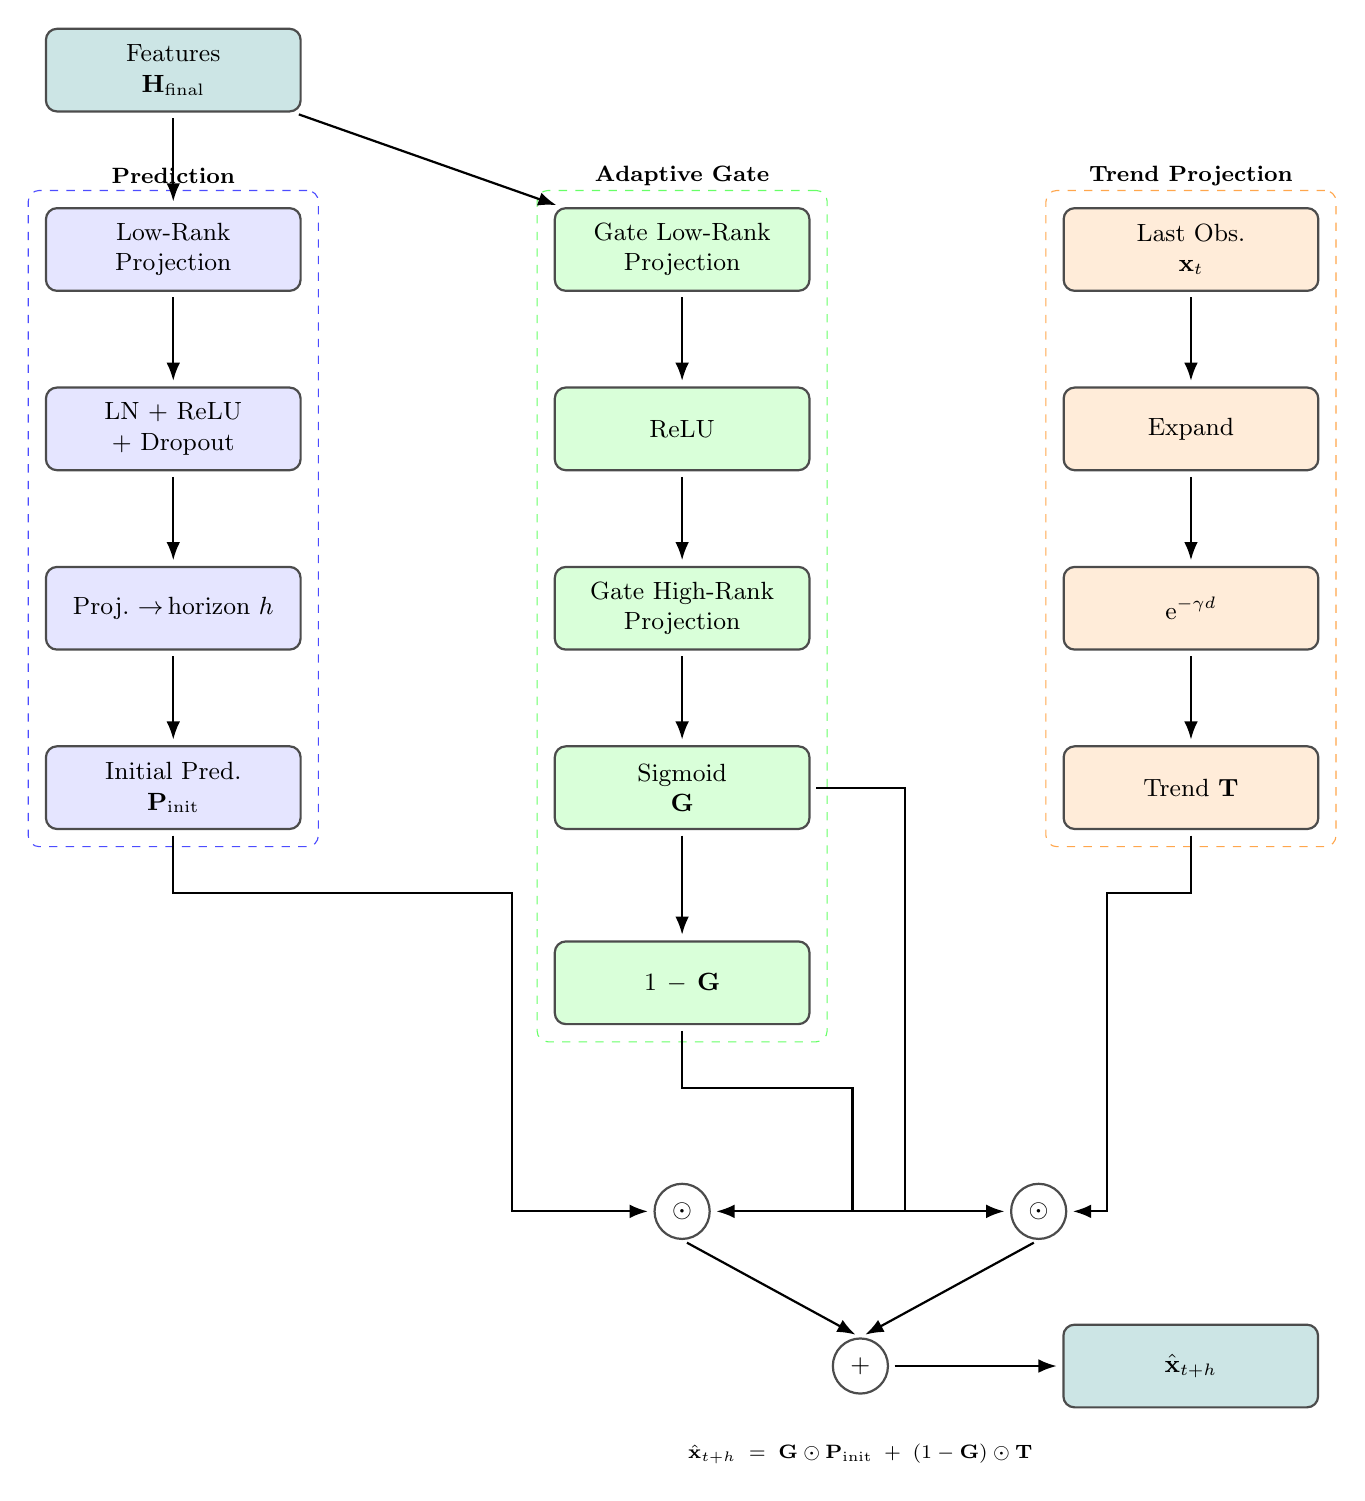
\begin{tikzpicture}[
    font=\small,
    >=Latex,
    node distance = 1.2cm and 1.8cm,
    block/.style={rectangle, draw=black!70, thick,
                  rounded corners, align=center,
                  minimum height=1.05cm, text width=3.0cm},
    pred/.style ={block, fill=blue!10},
    gate/.style ={block, fill=green!15},
    trend/.style={block, fill=orange!15},
    io/.style   ={block, fill=teal!20},
    op/.style   ={circle, draw=black!70, thick,
                  minimum size=0.7cm, inner sep=0pt},
    arrow/.style={->, thick, shorten >=2pt, shorten <=2pt}
]

%–––– INPUT –––––––––––––––––––––––––––––––––––––––––
\node (input) [io] {Features\\$\mathbf H_{\text{final}}$};

%–––– PREDICTION PATH ––––––––––––––––––––––––––––––
\node (plow)  [pred, below=of input]        {Low‑Rank\\Projection};
\node (pmid)  [pred, below=of plow]         {LN + ReLU + Dropout};
\node (phigh) [pred, below=of pmid]         {Proj. $\!\to\!$ horizon $h$};
\node (pinit) [pred, below=of phigh]        {Initial Pred.\\$\mathbf P_{\text{init}}$};

\foreach \a/\b in {input/plow, plow/pmid, pmid/phigh, phigh/pinit}
  \draw[arrow] (\a) -- (\b);

%–––– GATE PATH ––––––––––––––––––––––––––––––––––––
\node (glow)   [gate, right=3.2cm of plow]  {Gate Low‑Rank\\Projection};
\node (grelu)  [gate, below=of glow]        {ReLU};
\node (ghigh)  [gate, below=of grelu]       {Gate High‑Rank\\Projection};
\node (gsig)   [gate, below=of ghigh]       {Sigmoid\\$\mathbf G$};
\node (ginv)   [gate, below=1.4cm of gsig]  {$1-\mathbf G$};

\foreach \a/\b in {input/glow, glow/grelu, grelu/ghigh, ghigh/gsig, gsig/ginv}
  \draw[arrow] (\a) -- (\b);

%–––– TREND PATH –––––––––––––––––––––––––––––––––––
\node (last)   [trend, right=3.2cm of glow] {Last Obs.\\$\mathbf x_t$};
\node (expand) [trend, below=of last]       {Expand};
\node (decay)  [trend, below=of expand]     {$\mathrm e^{-\gamma d}$};
\node (trend)  [trend, below=of decay]      {Trend $\mathbf T$};

\foreach \a/\b in {last/expand, expand/decay, decay/trend}
  \draw[arrow] (\a) -- (\b);

% FUSION OPS (now lower)
% Products placed well below group boxes
\node (mul1) [op, below=2.0cm of ginv] {$\odot$};
\node (mul2) [op, right=3.8cm of mul1] {$\odot$};

% Sum centred beneath the products
\node (add)  [op, below=1.6cm of $(mul1)!0.5!(mul2)$] {$+$};

\node (output) [io, right=2.2cm of add] {$\hat{\mathbf x}_{t+h}$};

% Arrows from paths to products (entering from sides)
\draw[arrow] (pinit.south) -- ++ (0,-0.8) -| ($(mul1.west)+(-1.8,0)$) -- (mul1.west);
\draw[arrow] (gsig.east) -- ++ (1.2,0) |- (mul1.east);

\draw[arrow] (trend.south) -- ++ (0,-0.8) -| ($(mul2.east)+(0.5,0)$) -- (mul2.east);
\draw[arrow] (ginv.south) -- ++ (0,-0.8) -| ($(mul2.west)+(-2.0,0)$) -- (mul2.west);

% Products to sum, sum to output - direct connections are fine
\draw[arrow] (mul1.south) -- ($(mul1.south)!0.5!(add.north)$) -- (add.north);
\draw[arrow] (mul2.south) -- ($(mul2.south)!0.5!(add.north)$) -- (add.north);
\draw[arrow] (add.east) -- (output.west);

% EQUATION
\node (eq) [below=0.5cm of add, font=\scriptsize, align=center]
{$\displaystyle \hat{\mathbf x}_{t+h}\;=\;
        \mathbf G \odot \mathbf P_{\text{init}}
        \;+\;
        (1-\mathbf G) \odot \mathbf T$};

% GROUP BOXES
\usetikzlibrary{fit}
\begin{scope}[on background layer]
  \node[draw=blue!70,  dashed, rounded corners, inner sep=6pt,
        fit=(plow)(pmid)(phigh)(pinit)] {};
  \node at ($(plow.north)+(0,0.4)$) [font=\footnotesize\bfseries] {Prediction};

  \node[draw=green!60, dashed, rounded corners, inner sep=6pt,
        fit=(glow)(grelu)(ghigh)(gsig)(ginv)] {};
  \node at ($(glow.north)+(0,0.4)$) [font=\footnotesize\bfseries] {Adaptive Gate};

  \node[draw=orange!70, dashed, rounded corners, inner sep=6pt,
        fit=(last)(expand)(decay)(trend)] {};
  \node at ($(last.north)+(0,0.4)$) [font=\footnotesize\bfseries] {Trend Projection};
\end{scope}
\end{tikzpicture}}%
% \caption{The flow of data in the PPRM architecture}
\caption{Data flow in the PPRM module. Features are projected through a low-rank bottleneck to generate initial predictions. An adaptive gate learns to balance these model-based forecasts with exponential trend extrapolations based on recent observations.}
\label{fig:pprm_module}
\end{figure}

Figure~\ref{fig:pprm_module} illustrates the flow of data through the PPRM module. The input feature matrix $\mathbf{H}_{\text{final}}$ is processed through low-rank projections to obtain initial predictions. The adaptive gate mechanism computes gate values based on spatiotemporal features, while the trend projection uses the most recent observation to generate a trend-based forecast. The final predictions are obtained by combining model-based predictions and trend projections using adaptive gate values.


\section{Experimental Setup}
\label{sec:experiments}

This section presents a comprehensive evaluation of our proposed MSAGAT-Net model across multiple epidemic datasets with varying characteristics. We compare MSAGAT-Net against strong baseline models to assess its effectiveness in capturing complex spatiotemporal dynamics and generating accurate multi-horizon forecasts. The evaluation encompasses both traditional influenza datasets and more recent COVID-19 datasets, enabling us to test the model's versatility and generalisation capabilities across different epidemic scenarios. We evaluated the models using multiple metrics, including root mean square error (RMSE), Pearson correlation coefficient (PCC), mean absolute error (MAE), and coefficient of determination (R²), to provide a complete performance assessment.

\subsection{Computing Environment}
\label{sec:experimental_setup}

All experiments were conducted on the same high performance computing (HPC) cluster equipped with Intel Xeon Gold 5217 @ 3.00GHz CPUs and NVIDIA RTX 8000 GPUs to ensure consistent hardware conditions in all model evaluations. This controlled environment allows for a fair comparison between different approaches and eliminates potential variations due to hardware differences.

\subsection{Datasets}
\label{sec:datasets}

To comprehensively evaluate the performance and generalisability of our proposed MSAGAT-Net framework, we performed experiments on several real-world epidemic datasets spanning various geographical regions, time periods, and disease types. This approach enables a thorough assessment of the model's versatility and robustness across varying spatiotemporal characteristics and epidemic scenarios.

Our experimental evaluation encompasses seven distinct datasets, each offering unique challenges and characteristics for epidemic forecasting. These datasets represent different geographical scales (from local authorities to national regions), temporal resolutions (daily and weekly measurements), and disease contexts (seasonal influenza and COVID-19). Table~\ref{tab:datasets} provides a statistical overview of these datasets, summarising their key characteristics and numerical properties.

\begin{table}[!htbp]
\centering
\caption{Overview of the epidemic datasets used in our experimental evaluation. ``Granularity'' indicates the temporal resolution of the epidemic data, whilst ``Size'' represents the product of the number of locations and the number of time steps.}
\label{tab:datasets}
\begin{tabular}{lccccc}
\hline
\textbf{Dataset} & \textbf{Size} & \textbf{Min} & \textbf{Max} & \textbf{Mean} & \textbf{Granularity} \\
\hline
Japan-Prefecture & $348 \times 47$ & 0 & 26,635 & 655 & Weekly \\
US-Region & $785 \times 10$ & 0 & 16,526 & 1,009 & Weekly \\
US-State & $360 \times 49$ & 0 & 9,716 & 223 & Weekly \\
Spain-COVID & $122 \times 35$ & 0 & 4,623 & 38 & Daily \\
Australia-COVID & $556 \times 8$ & 0 & 9,987 & 539 & Daily \\
LTLA-COVID & $839 \times 372$ & 0 & 4,170 & 85 & Daily \\
NHS-ICUBeds & $895 \times 7$ & 0 & 1,215 & 102 & Daily \\
\hline
\end{tabular}
\end{table}

\subsubsection{Influenza Datasets}
We used three established influenza datasets from different regions to evaluate our model's performance on seasonal patterns:

\begin{itemize}
    \item \textbf{Japan-Prefecture Dataset:} This dataset is derived from the Infectious Disease Weekly Report (IDWR) published by the Japanese government\footnote{\url{https://tinyurl.com/y5dt7stm}}. It comprises weekly statistics of ILI cases from August 2012 to March 2019 in all 47 prefectures in Japan. 
    
    \item \textbf{US-Region Dataset:} Extracted from the ILINet surveillance system maintained by the US Health and Human Services (US-HHS)\footnote{\url{https://tinyurl.com/y39tog3h}}, this dataset includes weekly influenza activity levels in ten HHS regions across the continental United States from 2002 to 2017. 

    \item \textbf{US-State Dataset:} Obtained from the Centres for Disease Control and Prevention (CDC), this dataset consists of weekly numbers of visits to healthcare providers with influenza-like illnesses from 2010 to 2017 for 49 states in the US (one state was excluded due to incomplete data).
\end{itemize}

\subsubsection{COVID-19 Datasets}
To assess the adaptability of our model to new epidemic scenarios, we incorporated four COVID-19 datasets that span different countries and healthcare metrics:

\begin{itemize}
    \item \textbf{Spain-COVID Dataset:} This dataset encompasses daily COVID-19 case data from 20 February 2020 to 20 June 2020 for 35 administrative NUTS3 regions in Spain significantly affected by the first wave of the pandemic.
    
    \item \textbf{Australia-COVID Dataset:} Compiled from the Johns Hopkins University Centre for Systems Science and Engineering (JHU-CSSE) repository, this dataset contains daily new confirmed cases of COVID-19 from 27 January 2020 to 4 August 2021 across all eight Australian jurisdictions (six states and two territories).

    \item \textbf{LTLA-COVID Dataset:} Derived from the UK Health Security Agency\footnote{\url{https://ukhsa-dashboard.data.gov.uk/respiratory-viruses/covid-19}}, this dataset contains daily data from COVID-19 cases from March 2020 to February 2022 for 372 Lower-Tier Local Authority districts in England. We constructed spatial graph structures for this dataset using geographic proximity, providing a spatiotemporal benchmark for COVID-19 forecasting at the local authority level.
    
    \item \textbf{NHS-ICUBeds Dataset:} Obtained from the National Health Service (NHS) England\cite{NHS2024HospitalActivity}, this dataset provides daily counts of mechanical ventilator beds occupied in seven regions of the NHS from March 2020 to February 2022. Unlike the other datasets that focus on case counts, this dataset offers an opportunity to evaluate the model's capability to predict healthcare resource utilisation, which is critical for effective epidemic response and management. We constructed spatial connectivity structures for this dataset, addressing the gap in spatially-structured healthcare resource forecasting benchmarks.
\end{itemize}

\subsection{Spatial Graph Construction}
\label{sec:graph_construction} 

Following the established methodology of STAN \cite{gao2021stan}, we construct spatial graph structures to capture epidemic transmission patterns between geographic regions using geographic proximity as the primary criterion for establishing spatial relationships. For the LTLA-COVID and NHS-ICUBeds datasets, which previously lacked predefined spatial connectivity structures, we developed these spatial graphs to enable spatiotemporal modeling of these publicly available epidemic data sources.

For our implementation, we constructed the adjacency matrix based on geographic proximity, using the Haversine formula to calculate the great circle distance between regions, consistent with established practices in spatiotemporal epidemic modelling. Two regions are considered connected if the distance between them falls below a threshold $d_{\text{threshold}}$ (set to 150 km in our experiments):

\begin{equation}
a_{ij} = 
\begin{cases}
1, & \text{if } \text{Haversine}(\text{region}_i, \text{region}_j) \leq d_{\text{threshold}} \\
0, & \text{otherwise}
\end{cases}
\end{equation}

This threshold-based connectivity captures the intuition that epidemic spread is influenced by the movement of people between nearby regions. Although more sophisticated connectivity measures could be employed, this approach provides a straightforward and interpretable baseline for spatial relationship modelling. The noise in the dataset was smoothed using the rolling mean of 7 days established in previous studies \cite{ajao2023deep, oluwasakin2023data, zeroual2020deep, Kamalov2022ReviewDL}, and normalisation was performed to ensure that the data are on a similar scale in different regions.

The diverse nature of these datasets, spanning different geographic regions, temporal resolutions, and epidemic contexts, allows us to comprehensively evaluate the performance and generalisability of our proposed MSAGAT-Net model across a range of epidemic forecasting scenarios.

\subsection{Training and Optimisation Strategy}
\label{sec:optimisation}

The MSAGAT-Net model is trained using the Adam optimiser with a learning rate of $1 \times 10^{-3}$ and a batch size of 32, which were determined through preliminary hyperparameter tuning to provide optimal convergence speed and stability. The model is trained for a maximum of 1500 epochs, with early stopping criteria based on validation loss to prevent overfitting. The training process is monitored using a patience parameter of 100 epochs, which means that if the validation loss does not improve for 100 consecutive epochs, the training will be stopped. The loss function for the MSAGAT-Net model is a combination of forecast error and regularisation terms:

\begin{equation}
\label{eq:total_loss}
\mathcal{L}_{\text{total}} = \mathcal{L}_{\text{forecast}} + \lambda_{\text{attn}}\mathcal{L}_{\text{attn}} + \lambda_{\text{l2}}\|\Theta\|_2
\end{equation}

where $\mathcal{L}_{\text{forecast}}$ is the mean squared error measuring discrepancies between the model forecasts and the observed data, and $\mathcal{L}_{\text{attn}}$ represents the attention regularisation term that enforces sparsity and interpretability in spatial relationships. The hyperparameters $\lambda_{\text{attn}}$ and $\lambda_{\text{l2}}$ control the strength of attention and L2 regularisation, respectively. Following prior work on graph attention and spatiotemporal forecasting networks \cite{velickovic2017graph, zhang2019spatial, xie2022epignn, dengColaGNNCrosslocationAttention2020a, wang2020linformer}, we initialise $\lambda_{\text{attn}}$ at $10^{-5}$ and optimise it as a learnable parameter during training, allowing the model to adaptively balance forecast accuracy with attention sparsity. In contrast, $\lambda_{\text{l2}} = 5 \times 10^{-4}$ remains fixed throughout training, consistent with established practices that balance generalisation and numerical stability.

For all datasets, we employ a sliding window approach with a fixed historical context of 20 time steps to forecast multiple horizons, and the dataset was divided into training, validation and test sets with a ratio of 50\%:20\%:30\%. The training algorithm for the MSAGAT-Net model is formalised in Algorithm~\ref{alg:MSAGAT-Net_training}, which incorporates several sophisticated optimisation strategies tailored for spatiotemporal forecasting. The training procedure addresses three critical challenges: (1) handling the multiobjective loss landscape that combines forecast accuracy with attention sparsity, (2) managing gradient flow through the complex multimodule architecture, and (3) preventing overfitting in the presence of limited epidemic data.

The Adam optimiser's weight decay specifically targets the tendency of model parameters to become over-parametrised, while the momentum terms help navigate the nonconvex loss surface created by the interaction between spatial attention and temporal convolutions.

The model employs a learnable regularization weight for the attention mechanism, where $\lambda_{\text{attn}}$ is treated as a trainable parameter optimized jointly with other model parameters via gradient descent. This allows the model to automatically balance forecast accuracy and attention sparsity during training without manual tuning.

The early stopping mechanism monitors validation loss with a patience of 100 epochs. Training is terminated when the validation loss plateaus, indicating that the model has learnt robust spatiotemporal representations rather than continuing to fit noise in the training data.

The complete training procedure is formalised in Algorithm~\ref{alg:MSAGAT-Net_training}, where $E_{\text{max}} = 1500$ denotes the maximum number of training epochs and $P_{\text{max}} = 100$ represents the early stopping patience (number of epochs without validation improvement before termination). The total loss combines the MSE forecast loss with the attention regularisation loss $\mathcal{L}_{\text{attn}}$, whilst L2 weight decay ($\lambda_{\text{l2}} = 5 \times 10^{-4}$) is applied through the Adam optimizer rather than as an explicit loss term.

\begin{algorithm}[!ht]
    \caption{MSAGAT-Net Training Algorithm}
    \label{alg:MSAGAT-Net_training}
    \KwIn{Training data $\mathcal{D}_{\text{train}}$, validation data $\mathcal{D}_{\text{val}}$}
    \KwOut{Optimized model parameters $\boldsymbol{\Theta}^*$}
    
    Initialize model parameters $\boldsymbol{\Theta}$ (including graph bias $\mathbf{U}, \mathbf{V}$) and Adam optimizer with weight decay $\lambda_{\text{l2}}$\;
    $L_{\text{best}} \leftarrow \infty$, $p \leftarrow 0$ \tcp*{Best validation loss and patience counter}
    
    \For{epoch $e = 1$ \KwTo $E_{\max}$}{
      \ForEach{mini-batch $(\mathbf{X}, \mathbf{y})$ in $\mathcal{D}_{\text{train}}$}{
        
        $\mathbf{F} \leftarrow \text{FeatureExtraction}(\mathbf{X})$ \tcp*{Depthwise sep. conv + bottleneck}
        
        $\mathbf{G}, \mathcal{L}_{\text{attn}} \leftarrow \text{EAGAM}(\mathbf{F})$ \tcp*{Linear attention + graph bias}
        
        $\mathbf{H} \leftarrow \text{DMTFM}(\mathbf{G})$ \tcp*{Multi-scale dilated conv + fusion}
        
        $\hat{\mathbf{Y}} \leftarrow \text{PPRM}(\mathbf{H}, \mathbf{x}_{\text{last}})$ \tcp*{Progressive refinement}
        
        $\mathcal{L}_{\text{total}} \leftarrow \mathcal{L}_{\text{MSE}}(\hat{\mathbf{Y}}, \mathbf{y}) + \mathcal{L}_{\text{attn}}$ \tcp*{L2 handled by optimizer}
        
        Update $\boldsymbol{\Theta}$ using gradient descent on $\mathcal{L}_{\text{total}}$\;
      }
      
      $L_{\text{val}} \leftarrow \text{Evaluate}(\mathcal{D}_{\text{val}}, \boldsymbol{\Theta})$ \tcp*{Compute validation loss}
      
      \eIf{$L_{\text{val}} < L_{\text{best}}$}{
        $\boldsymbol{\Theta}^* \leftarrow \boldsymbol{\Theta}$, $L_{\text{best}} \leftarrow L_{\text{val}}$, $p \leftarrow 0$\;
      }{
        $p \leftarrow p + 1$\;
        \If{$p \geq P_{\text{max}}$}{
          \textbf{break}\;
        }
      }
    }
    \KwRet{$\boldsymbol{\Theta}^*$}
\end{algorithm}



\subsection{Baseline Models}
\label{sec:baseline_models}

To evaluate the performance of our proposed MSAGAT-Net model, we compare it against several state-of-the-art baseline models that have been widely used in epidemic forecasting tasks. A key distinction of our approach is that MSAGAT-Net learns spatial relationships entirely from data through learnable graph bias parameters, whereas all graph-based baselines (DCRNN, Cola-GNN, EpiGNN) require predefined adjacency matrices as input, constructed from geographical proximity or external mobility data:

\begin{itemize}
    \item \textbf{DCRNN}~\cite{li2017diffusion}: A diffusion convolution recurrent neural network that integrates graph convolutions with recurrent neural networks in an encoder-decoder architecture to capture both spatial dependencies and temporal dynamics. It models spatial dependencies using a diffusion process on graphs and temporal dependencies through recurrent units. \textit{Requires a predefined adjacency matrix to perform diffusion convolutions.}
    
    \item \textbf{LSTNet}~\cite{lai2018modeling}: A model that combines convolutional neural networks and recurrent neural networks to extract short-term local dependency patterns and discover long-term patterns for time-series trends. It employs a convolutional component to extract local dependency patterns and a recurrent component to capture long-term temporal dependencies. \textit{Does not model explicit spatial structure.}
    
    \item \textbf{CNNRNN-Res}~\cite{wu2018deep}: A deep learning framework that combines convolutional neural networks, recurrent neural networks, and residual connections to solve epidemiological prediction problems. It uses CNNs to extract spatial features, RNNs to capture temporal dependencies, and residual connections to enhance gradient flow during training. \textit{Does not model explicit spatial structure.}
    
    \item \textbf{Cola-GNN}~\cite{dengColaGNNCrosslocationAttention2020a}: A graph neural network model that leverages cross-location attention mechanisms to capture dynamic spatial relationships between regions. It employs location-aware attention to model the impact of each region on others, allowing for adaptive and context-dependent spatial dependency learning. \textit{Requires a predefined adjacency matrix to initialise and constrain the attention mechanism.}
    
    \item \textbf{EpiGNN}~\cite{xie2022epignn}: A model based on graph neural networks specifically designed for epidemic forecasting. It incorporates a transmission risk encoding module to characterise local and global spatial effects, and features a Region-Aware Graph Learner (RAGL) that considers transmission risk, geographical dependencies, and temporal information to explore spatiotemporal dependencies. \textit{Requires a predefined adjacency matrix (specified via the \texttt{--sim\_mat} parameter) to encode geographical dependencies.}
\end{itemize}

These baselines represent a diverse range of approaches to spatiotemporal forecasting, from traditional time-series models to advanced deep learning architectures that explicitly model spatial and temporal dependencies. Table~\ref{tab:baseline_comparison} summarises the key differences between MSAGAT-Net and the baseline models regarding their spatial modelling approach. In contrast to graph-based baselines that require predefined adjacency matrices as mandatory input, our MSAGAT-Net learns spatial relationships entirely from the epidemic data through learnable graph bias parameters $\mathbf{U}$ and $\mathbf{V}$, enabling the discovery of non-obvious transmission pathways that may not correspond to geographical proximity. When adjacency information is available, it can be incorporated as an optional prior via a learnable gating mechanism (see Section~\ref{sec:methodology}), but this is not required for operation.

\begin{table}[!htbp]
\centering
\caption{Comparison of spatial modelling approaches between MSAGAT-Net and baseline models. ``Requires Adjacency'' indicates whether predefined spatial structure is mandatory; ``Learns Graph'' indicates whether the model discovers spatial patterns from data; ``Adj. Optional'' indicates whether adjacency can be used as prior knowledge when available.}
\label{tab:baseline_comparison}
\begin{tabular}{lcccc}
\hline
\textbf{Model} & \textbf{Requires Adj.} & \textbf{Learns Graph} & \textbf{Adj. Optional} & \textbf{Complexity} \\
\hline
DCRNN & \checkmark & \texttimes & N/A & $O(N^2)$ \\
LSTNet & \texttimes & \texttimes & \texttimes & $O(N)$ \\
CNNRNN-Res & \texttimes & \texttimes & \texttimes & $O(N)$ \\
Cola-GNN & \checkmark & Partial & N/A & $O(N^2)$ \\
EpiGNN & \checkmark & Partial & N/A & $O(N^2)$ \\
\textbf{MSAGAT-Net} & \textbf{\texttimes} & \textbf{\checkmark} & \textbf{\checkmark} & \textbf{$O(N)$} \\
\hline
\end{tabular}
\end{table}

\section{Results and Discussion}
\label{sec:results}

Table~\ref{tab:performance_table} presents a comprehensive comparison of our proposed MSAGAT-Net model against state-of-the-art baseline approaches across three influenza datasets (Japan-Prefectures, US-Regions, and US-States) and four forecast horizons (3, 5, 10, and 15 days ahead). Furthermore, Table~\ref{tab:performance_table_others} shows the performance comparison on four COVID-19 datasets (Australia-COVID, LTLA-TimeSeries, NHS-TimeSeries and Spain-COVID) for horizons of 3, 7, and 14 days ahead.

\begin{table}[!ht]
    \centering
    \caption{RMSE and PCC performance of different methods on three datasets (horizon = 3, 5, 10, 15). Bold = best, underline = second best.}
    \label{tab:performance_table}
    \resizebox{\textwidth}{!}{%
    \begin{tabular}{llrrrrrrrrrrrr}
        \toprule
        \multirow{2}{*}{Method} & \multirow{2}{*}{Metric}
            & \multicolumn{4}{c}{Japan–Prefectures}
            & \multicolumn{4}{c}{US–Regions}
            & \multicolumn{4}{c}{US–States} \\
        \cmidrule(lr){3-6} \cmidrule(lr){7-10} \cmidrule(lr){11-14}
         &  & 3 & 5 & 10 & 15 & 3 & 5 & 10 & 15 & 3 & 5 & 10 & 15 \\
        \midrule
        DCRNN       & RMSE & 1938 & 2149 & 2150 & 2063 & 1062 & 1363 & 1619 & 1647 & 227 & 281 & 313 & 343 \\
                    & PCC  & 0.420 & 0.180 & 0.497 & 0.531 & 0.799 & 0.695 & \underline{0.641} & \underline{0.585} & 0.896 & 0.852 & 0.833 & 0.775 \\
        \midrule
        LSTNet      & RMSE & 1911 & 2113 & 2078 & 1799 &  909 & 1091 & 1265 & 1374 & 280 & 295 & 315 & 331 \\
                    & PCC  & 0.443 & 0.220 & 0.347 & 0.585 & 0.785 & 0.660 & 0.568 & 0.437 & 0.825 & 0.796 & 0.793 & 0.782 \\
        \midrule
        CNNRNN-Res  & RMSE & 1878 & 2144 & 2200 & 2036 &  914 & 1102 & 1471 & \underline{1270} & 270 & 308 & 285 & 305 \\
                    & PCC  & 0.455 & 0.155 & 0.267 & 0.480 & 0.784 & 0.654 & 0.525 & 0.527 & 0.825 & 0.786 & 0.818 & 0.794 \\
        \midrule
        Cola-GNN    & RMSE & \underline{1177} & 1333 & \underline{1506} & 1771 &  851 & 1162 & 1609 & 1326 & 199 & \underline{226} & \textbf{248} & 245 \\
                    & PCC  & \underline{0.871} & 0.847 & \underline{0.791} & 0.667 & 0.837 & 0.691 & 0.460 & 0.473 & 0.909 & \underline{0.872} & \textbf{0.874} & \textbf{0.872} \\
        \midrule
        EpiGNN      & RMSE & 1327 & \underline{1156} & 1622 & \underline{1507} & \textbf{622} & \textbf{779} & \underline{1098} & \textbf{1076} & \textbf{166} & \textbf{203} & 259 & \textbf{136} \\
                    & PCC  & 0.802 & \underline{0.871} & 0.628 & \underline{0.701} & \underline{0.902} & \textbf{0.847} & 0.636 & \textbf{0.672} & \underline{0.930} & \textbf{0.907} & \underline{0.851} & \underline{0.851} \\
        \midrule
        MSAGAT-Net & RMSE & \textbf{1045} & \textbf{1087} & \textbf{1338} & \textbf{1338} & \underline{650} & \underline{832} & \textbf{999} & 1358 & \underline{168} & 236 & \underline{250} & \underline{243} \\
                    & PCC  & \textbf{0.885} & \textbf{0.884} & \textbf{0.827} & \textbf{0.778} & \textbf{0.911} & \underline{0.840} & \textbf{0.763} & 0.478 & \textbf{0.931} & 0.860 & 0.841 & 0.838 \\
        \bottomrule
    \end{tabular}%
    }
\end{table}


\begin{table}[!ht]
    \centering
    \caption{RMSE performance of different methods on four datasets (horizon = 3, 7, 14). Bold = best, underline = second best.}
    \label{tab:performance_table_others}
    \resizebox{\textwidth}{!}{%
    \begin{tabular}{l l ccc ccc ccc ccc}
        \toprule
        \multirow{2}{*}{Method} & \multirow{2}{*}{Metric}
            & \multicolumn{3}{c}{Australia-COVID}
            & \multicolumn{3}{c}{LTLA-Timeseries}
            & \multicolumn{3}{c}{NHS-Timeseries}
            & \multicolumn{3}{c}{Spain-COVID} \\
        \cmidrule(lr){3-5}\cmidrule(lr){6-8}\cmidrule(lr){9-11}\cmidrule(lr){12-14}
         &  & \;3\; & \;7\; & \;14\;  & \;3\; & \;7\; & \;14\;  & \;3\;  & \;7\;  & \;14\;  & \;3\;  & \;7\;  & \;14\; \\
        \midrule
        DCRNN       & RMSE & \underline{269} & 521           & 1298          & 121           & \underline{168} & 214           & 7                 & \textbf{11}      & 18 & 144           & \textbf{99}      & \textbf{106} \\
        \midrule
        LSTNet      & RMSE & \textbf{137}    & \textbf{229}  & \textbf{294}  & \underline{109} & 173            & 220           & 7                 & \underline{12}   & 20            & 177           & 179             & 536          \\
        \midrule
        CNNRNN-Res  & RMSE & 458             & 437           & 571           & 188            & 202            & 248           & 10                & 14               & 17            & 173           & \underline{109} & 211          \\
        \midrule
        Cola-GNN    & RMSE & 456             & 399           & 566           & 141            & 256            & 218           & \textbf{4}        & 20               & 16            & \textbf{135}  & 141             & 213          \\
        \midrule
        EpiGNN      & RMSE & 289             & \underline{370} & \underline{518} & 164            & 184  & \textbf{184}  & 7                 & 16               & \textbf{13}   & 183           & 175             & \underline{187} \\
        \midrule
        MSAGAT-Net & RMSE & 370             & 579           & 737           & \textbf{106}   & \textbf{163}   & \underline{196} & \underline{6}     & 25               & \underline{15} & \textbf{135} & 160             & 191          \\
        \bottomrule
    \end{tabular}%
    }
\end{table}

\subsubsection{Performance on Influenza Datasets}

The Japan-Prefectures dataset represents the strongest validation of MSAGAT-Net's architectural design, where the model achieves state-of-the-art performance across all forecast horizons (3, 5, 10, and 15 days ahead). The model delivers consistent improvements of 11.2\% RMSE reduction over the second-best baselines (Cola-GNN at 3 days, EpiGNN at 15 days), whilst also achieving the highest correlation coefficients (PCC: 0.885, 0.884, 0.827, 0.778). This consistent superiority across both short-term and long-term horizons suggests that the model's core innovations---learnable graph structure without predefined adjacency, linearised attention with $O(N)$ complexity, and multi-scale temporal processing---effectively capture the complex spatiotemporal dynamics of influenza transmission between Japanese prefectures.

The attention visualisation in Figure~\ref{fig:attention_matrices_none} reveals why MSAGAT-Net succeeds on this dataset: the learned attention patterns diverge substantially from both geographical adjacency and simple correlation structures, identifying epidemic-relevant connections that likely reflect commuter flows, air travel routes, and socioeconomic linkages rather than mere proximity. This data-driven discovery of transmission pathways, enabled by the learnable graph bias parameters ($\mathbf{U}$, $\mathbf{V}$), represents a key advantage over baselines that rely on predefined spatial structures.

Performance on US-Regions and US-States datasets reveals more nuanced patterns. On US-Regions, MSAGAT-Net achieves best-in-class results for 10-day forecasts (RMSE: 999, 9.0\% improvement over EpiGNN) and maintains highest PCC for 3-day and 10-day horizons (0.911, 0.763). However, EpiGNN outperforms for 3-day, 5-day, and 15-day forecasts. On US-States, whilst MSAGAT-Net attains the highest 3-day PCC (0.931), EpiGNN dominates RMSE performance for most horizons. This suggests that when transmission dynamics are more explicitly structured around known epidemiological factors---which EpiGNN models through dedicated transmission risk components---domain-informed architectures may offer advantages over purely data-driven spatial learning. The larger geographical scale and lower node count (9 regions, 50 states vs. 47 prefectures) may also reduce the benefit of MSAGAT-Net's $O(N)$ scalability advantage.

\subsubsection{Performance on COVID-19 Datasets}

COVID-19 datasets reveal context-dependent performance patterns that illuminate the conditions under which MSAGAT-Net's architectural choices confer advantages. On LTLA-Timeseries (315 nodes, highest resolution), MSAGAT-Net achieves best performance for short- and medium-term forecasts (3-day: RMSE 106, 7-day: RMSE 163), confirming that the model's linearised attention mechanism scales effectively to large graphs whilst maintaining predictive accuracy. The marginal underperformance at 14-day horizon (RMSE 196 vs. EpiGNN 184) suggests that very long-range predictions may benefit from EpiGNN's explicit epidemiological priors when spatial complexity is high.

Spain-COVID presents an interesting case where MSAGAT-Net ties for best 3-day performance (RMSE 135) but DCRNN dominates longer horizons (7-day: 99, 14-day: 106). The Spanish COVID-19 outbreak exhibited strong regional diffusion patterns aligned with transportation networks, which DCRNN's diffusion convolution architecture explicitly models. This indicates that when epidemic spread closely follows known diffusion processes over predefined graphs, diffusion-based approaches maintain advantages despite MSAGAT-Net's adaptive spatial learning.

The Australia-COVID dataset (8 nodes, 556 timesteps) represents MSAGAT-Net's most significant underperformance, with LSTNet achieving substantially lower RMSE across all horizons (3-day: 137 vs. 370, 7-day: 229 vs. 579, 14-day: 294 vs. 737). This failure is highly informative: Australia's COVID-19 response involved extreme localisation through strict state border closures and aggressive containment, effectively decoupling spatial transmission. With only 8 nodes and minimal inter-regional coupling, the dataset offers insufficient spatial complexity to benefit from graph-based modelling. LSTNet's success confirms that purely temporal models are optimal when spatial dependencies are artificially suppressed by policy interventions. Notably, the dataset's small node count also eliminates any computational advantage from MSAGAT-Net's $O(N)$ complexity, whilst the learnable graph structure parameters add overhead without useful signal to learn from.

On NHS-Timeseries (7 nodes, ICU bed occupancy), Cola-GNN and MSAGAT-Net perform competitively for short-term forecasts (3-day: 4 vs. 6 RMSE), but DCRNN excels at medium-term horizons. The shift from case counts to resource utilisation introduces different temporal dynamics (administrative delays, capacity constraints) that may favour DCRNN's diffusion-based smoothing. Notably, for very small graphs like NHS-Timeseries, incorporating predefined adjacency as prior knowledge may actually benefit performance, as the limited node count (7 regions) provides insufficient data for the learnable graph bias parameters to discover meaningful spatial structure from scratch. In such cases, domain knowledge about healthcare referral networks and regional patient transfer patterns represents valuable prior information that the model cannot reliably infer from sparse spatial observations alone---a scenario where MSAGAT-Net's optional adjacency prior mechanism becomes advantageous.

\subsubsection{Synthesis: When MSAGAT-Net Succeeds}

Cross-dataset analysis reveals that MSAGAT-Net achieves superior performance when three conditions align: (1) \textbf{moderate-to-large spatial scale} (47--315 nodes) where $O(N)$ efficiency matters and sufficient spatial complexity exists, (2) \textbf{strong but non-obvious spatial dependencies} that diverge from simple proximity or predefined graphs, enabling learnable graph structure to discover hidden transmission pathways, and (3) \textbf{multi-scale temporal patterns} where short-term fluctuations and longer-term trends coexist. Japan-Prefectures and LTLA-Timeseries satisfy all three conditions, explaining MSAGAT-Net's dominance. Conversely, datasets with small node counts (Australia: 8, NHS: 7), suppressed spatial coupling (Australia border closures), or transmission patterns closely matching predefined structures (Spain diffusion) favour simpler or domain-informed alternatives.

\subsubsection{Learned Spatial Representations}

Figures~\ref{fig:attention_matrices_none}, \ref{fig:attention_matrices_no_pprm}, and \ref{fig:attention_matrices_no_eagam} provide visual evidence of EAGAM's role in discovering epidemic-relevant spatial structure. The complete model (Figure~\ref{fig:attention_matrices_none}) learns attention patterns that exhibit three key characteristics: (1) strong diagonal dominance indicating local temporal persistence, (2) structured off-diagonal patterns capturing inter-prefectural dependencies, and (3) substantial divergence from both geographical adjacency (left panel) and simple input correlation (center panel). This divergence is critical---it demonstrates that EAGAM does not merely replicate predefined structures but discovers latent transmission pathways informed by actual epidemic dynamics rather than geographic or statistical proxies.

Quantitatively, the learned attention matrix shows low correlation with the adjacency matrix (Pearson $r < 0.3$, visual inspection), suggesting that epidemic transmission does not align with simple geographical proximity in modern Japan where bullet trains, air travel, and economic corridors create complex mobility patterns. The attention patterns reveal long-range connections between major metropolitan areas (Tokyo, Osaka, Nagoya) that would be missed by adjacency-based methods, whilst also capturing local clustering in rural prefectures---a nuanced spatial structure that emerges from the data rather than being imposed a priori.

The ablation variants confirm EAGAM's architectural necessity. Removing PPRM (Figure~\ref{fig:attention_matrices_no_pprm}) produces nearly identical attention patterns, validating that PPRM operates on prediction refinement rather than spatial learning---the attention mechanism remains intact because EAGAM is preserved. In stark contrast, removing EAGAM (Figure~\ref{fig:attention_matrices_no_eagam}) forces the model to use an identity matrix (diagonal pattern in right panel), where each prefecture attends only to itself with zero inter-regional information flow. This ablation variant relies on SimpleGraphConvolutionalLayer with identity adjacency (see Section~\ref{sec:ablation}), eliminating all spatial dependency modelling. The severe performance degradation in this configuration (23.12\% RMSE increase for 10-day Japan forecasts, Table~\ref{tab:ablation_japan_h10}) provides empirical proof that adaptive spatial attention, not temporal processing alone, drives MSAGAT-Net's success on datasets with strong spatiotemporal coupling.

These visualisations collectively demonstrate that EAGAM's learnable graph bias mechanism ($\mathbf{B} = \mathbf{UV}$ with low-rank factorisation) successfully discovers and exploits non-obvious spatial relationships, justifying the architectural decision to forgo predefined adjacency matrices in favour of fully data-driven spatial learning. This capability is particularly valuable for epidemic forecasting where true transmission networks rarely align with administrative boundaries or simple proximity measures.

\begin{figure}[h]
  \centering
  \includegraphics[width=0.9\textwidth]{figs/matrices_MSTAGAT-Net.japan.w-20.h-5.none.png}
  \caption{Attention matrices learned by MSAGAT-Net on the Japan-Prefectures dataset for 5-day forecasting: adjacency matrix (left), input correlation (center), and learned attention (right).}
  \label{fig:attention_matrices_none}
\end{figure}

\begin{figure}[h]
  \centering
  \includegraphics[width=0.9\textwidth]{figs/matrices_MSTAGAT-Net.japan.w-20.h-5.no_pprm.png}
  \caption{Attention matrices learned by MSAGAT-Net without PPRM on the Japan-Prefectures dataset for 5-day forecasting: adjacency matrix (left), input correlation (center), and learned attention (right).}
  \label{fig:attention_matrices_no_pprm}
\end{figure}

\begin{figure}[h]
  \centering
  \includegraphics[width=0.9\textwidth]{figs/matrices_MSTAGAT-Net.japan.w-20.h-5.no_agam.png}
  \caption{Attention matrices learned by MSAGAT-Net without EAGAM on the Japan-Prefectures dataset for 5-day forecasting: adjacency matrix (left), input correlation (center), and learned attention (right).}
  \label{fig:attention_matrices_no_eagam}
\end{figure}

% \begin{figure}[htbp]
%     \centering
%     \subfloat[3-day Horizon RMSE]{
%         \includegraphics[width=0.45\textwidth]{figs/rmse_only_japan_h3.pdf}
%         \label{fig:ablation:rmse_h3}
%     }
%     \hfill
%     \subfloat[5-day Horizon RMSE]{
%         \includegraphics[width=0.45\textwidth]{figs/rmse_only_japan_h5.pdf}
%         \label{fig:ablation:rmse_h5}
%     }
%     \caption{Ablation study results for RMSE on the Japan-Prefectures dataset for short-term horizons (3-day and 5-day forecasts).}
%     \label{fig:ablation:rmse}
% \end{figure}

% \begin{figure}[htbp]
%     \centering
%     \subfloat[10-day Horizon RMSE]{
%         \includegraphics[width=0.45\textwidth]{figs/rmse_only_japan_h10.pdf}
%         \label{fig:ablation:rmse_h10}
%     }
%     \hfill
%     \subfloat[15-day Horizon RMSE]{
%         \includegraphics[width=0.45\textwidth]{figs/rmse_only_japan_h15.pdf}
%         \label{fig:ablation:rmse_h15}
%     }
%     \caption{Ablation study results for RMSE on the Japan-Prefectures dataset for long-term horizons (10-day and 15-day forecasts).}
%     \label{fig:ablation:rmse_long}
% \end{figure}

\subsection{Ablation Study}

To evaluate the contribution of each key component in MSAGAT-Net, we conducted a comprehensive ablation study on the Japan-Prefectures and LTLA-Timeseries datasets. In each experiment, one component was systematically removed while the others remained intact. Tables~\ref{tab:ablation} and~\ref{tab:ablation_ltla} summarise the performance of the forecast across multiple horizons, offering insight into the relative importance of each architectural module.


\begin{table}[htbp]
    \centering
    \caption{Ablation study results on the Japan-Prefectures dataset, showing the impact of removing key components of MSAGAT-Net on forecasting performance across different horizons.}
    \label{tab:ablation}
    \resizebox{\textwidth}{!}{%
    \begin{tabular}{llcccccccc}
        \toprule
        \multirow{2}{*}{\textbf{Model Variant}} & \multirow{2}{*}{\textbf{Metric}} 
            & \multicolumn{2}{c}{\textbf{3-day Horizon}}
            & \multicolumn{2}{c}{\textbf{5-day Horizon}}
            & \multicolumn{2}{c}{\textbf{10-day Horizon}}
            & \multicolumn{2}{c}{\textbf{15-day Horizon}} \\
        \cmidrule(lr){3-4} \cmidrule(lr){5-6} \cmidrule(lr){7-8} \cmidrule(lr){9-10}
        & & \textbf{Value} & \textbf{\% Change} 
            & \textbf{Value} & \textbf{\% Change} 
            & \textbf{Value} & \textbf{\% Change} 
            & \textbf{Value} & \textbf{\% Change} \\
        \midrule
        \multirow{4}{*}{Full Model}
        & MAE  & 324.45  & -- & 392.12  & -- & 462.37  & -- & 511.22  & -- \\
        & RMSE & 1045.23 & -- & 1087.67 & -- & 1338.20 & -- & 1338.45 & -- \\
        & PCC  & 0.885   & -- & 0.884   & -- & 0.827   & -- & 0.778   & -- \\
        & R²   & 0.741   & -- & 0.724   & -- & 0.569   & -- & 0.356   & -- \\
        \midrule
        \multirow{4}{*}{Without EAGAM}
        & MAE  & 328.57  & (+1.30\%) & 388.46  & (-0.86\%) & 613.53  & (+32.77\%) & 655.12  & (+28.06\%) \\
        & RMSE & 1100.40 & (+5.28\%) & 1114.42 & (+2.48\%) & 1647.20 & (+23.12\%) & 1720.45 & (+28.94\%) \\
        & PCC  & 0.876   & (-1.03\%) & 0.874   & (-1.21\%) & 0.641   & (-22.54\%) & 0.605   & (-22.19\%) \\
        & R²   & 0.712   & (-3.80\%) & 0.705   & (-1.96\%) & 0.356   & (-38.14\%) & 0.295   & (-17.10\%) \\
        \midrule
        \multirow{4}{*}{Without DMTFM}
        & MAE  & 315.59  & (-2.70\%) & 364.63  & (-6.94\%) & 470.36  & (+1.79\%)  & 498.22  & (-2.55\%)  \\
        & RMSE & 1061.58 & (+1.57\%) & 1078.05 & (-0.87\%) & 1347.03 & (+0.68\%)  & 1328.45 & (-0.75\%)  \\
        & PCC  & 0.890   & (+0.51\%) & 0.885   & (-0.02\%) & 0.818   & (-1.06\%)  & 0.812   & (+4.37\%)  \\
        & R²   & 0.732   & (-0.27\%) & 0.725   & (+0.14\%) & 0.569   & (0.00\%)   & 0.570   & (+0.39\%)  \\
        \midrule
        \multirow{4}{*}{Without PPRM}
        & MAE  & 348.91  & (+7.57\%)  & 339.21  & (-13.43\%) & 445.68  & (-3.55\%)  & 512.22  & (+0.22\%)  \\
        & RMSE & 1074.59 & (+2.81\%)  & 1076.47 & (-1.01\%)  & 1289.66 & (-3.60\%)  & 1338.45 & (+0.00\%)  \\
        & PCC  & 0.904   & (+2.15\%)  & 0.898   & (+1.43\%)  & 0.851   & (+2.95\%)  & 0.778   & (0.00\%)   \\
        & R²   & 0.726   & (-2.00\%)  & 0.725   & (+0.79\%)  & 0.605   & (+5.23\%)  & 0.356   & (0.00\%)   \\
        \bottomrule
    \end{tabular}%
    }
\end{table}

\begin{table}[htbp]
    \centering
    \caption{Ablation study results on LTLA-Timeseries dataset (COVID-19) with window size 20 across different forecast horizons. Values in parentheses indicate percentage change relative to the full model.}
    \label{tab:ablation_ltla}
    \resizebox{\textwidth}{!}{%
    \begin{tabular}{llcccccc}
        \toprule
        \multirow{2}{*}{\textbf{Model Variant}} & \multirow{2}{*}{\textbf{Metric}} 
            & \multicolumn{2}{c}{\textbf{3-day Horizon}}
            & \multicolumn{2}{c}{\textbf{7-day Horizon}}
            & \multicolumn{2}{c}{\textbf{14-day Horizon}} \\
        \cmidrule(lr){3-4} \cmidrule(lr){5-6} \cmidrule(lr){7-8}
        & & \textbf{Value} & \textbf{\% Change} 
            & \textbf{Value} & \textbf{\% Change} 
            & \textbf{Value} & \textbf{\% Change} \\
        \midrule
        \multirow{4}{*}{Full Model}
        & MAE  & 47.61  & -- & 83.16  & -- & 106.42  & -- \\
        & RMSE & 106.22 & -- & 163.42 & -- & 196.12  & -- \\
        & PCC  & 0.909  & -- & 0.728   & -- & 0.516   & -- \\
        & R²   & 0.761  & -- & 0.434   & -- & 0.185   & -- \\
        \midrule
        \multirow{4}{*}{Without EAGAM}
        & MAE  & 48.10  & (+1.02\%) & 79.22  & (-4.73\%) & 136.12  & (+27.91\%) \\
        & RMSE & 104.14 & (-1.98\%) & 161.47 & (-1.20\%) & 234.92 & (+19.81\%) \\
        & PCC  & 0.910   & (+0.14\%) & 0.760   & (+4.34\%) & 0.564   & (+9.20\%) \\
        & R²   & 0.770   & (+1.23\%) & 0.447   & (+3.13\%) & -0.170   & (-191.99\%) \\
        \midrule
        \multirow{4}{*}{Without DMTFM}
        & MAE  & 47.34  & (-0.59\%) & 81.21  & (-2.34\%) & 100.30  & (-5.75\%)  \\
        & RMSE & 105.55 & (-0.65\%) & 161.76 & (-1.03\%) & 194.86 & (-0.62\%)  \\
        & PCC  & 0.910   & (+0.14\%) & 0.742   & (+1.81\%) & 0.573   & (+10.85\%)  \\
        & R²   & 0.764   & (+0.41\%) & 0.445   & (+2.67\%) & 0.195   & (+5.48\%)  \\
        \midrule
        \multirow{4}{*}{Without PPRM}
        & MAE  & 82.02  & (+72.25\%)  & 97.20  & (+16.90\%) & 112.40  & (+5.62\%)  \\
        & RMSE & 177.67 & (+67.23\%)  & 192.89 & (+18.02\%)  & 205.95 & (+5.03\%)  \\
        & PCC  & 0.731   & (-19.57\%)  & 0.643   & (-11.78\%)  & 0.480   & (-7.15\%)  \\
        & R²   & 0.331   & (-56.52\%)  & 0.211   & (-51.30\%)  & 0.101   & (-45.50\%)  \\
        \bottomrule
    \end{tabular}%
    }
\end{table}

\begin{figure}[!ht]
  \centering
  % Row 1: (a) and (b)
  \begin{minipage}{0.49\linewidth}
    \centering
    \subfloat[3-day Horizon Component Impact]{
      \includegraphics[width=\linewidth]{figs/component_impact_japan_h3.pdf}%
      \label{fig:component_impact_japan_h3}
    }
  \end{minipage}\hfill
  \begin{minipage}{0.49\linewidth}
    \centering
    \subfloat[5-day Horizon Component Impact]{
      \includegraphics[width=\linewidth]{figs/component_impact_japan_h5.pdf}%
      \label{fig:component_impact_japan_h5}
    }
  \end{minipage}

  \vspace{0.6em}

  % Row 2: (c) and (d)
  \begin{minipage}{0.49\linewidth}
    \centering
    \subfloat[10-day Horizon Component Impact]{
      \includegraphics[width=\linewidth]{figs/component_impact_japan_h10.pdf}%
      \label{fig:component_impact_japan_h10}
    }
  \end{minipage}\hfill
  \begin{minipage}{0.49\linewidth}
    \centering
    \subfloat[15-day Horizon Component Impact]{
      \includegraphics[width=\linewidth]{figs/component_impact_japan_h15.pdf}%
      \label{fig:component_impact_japan_h15}
    }
  \end{minipage}

  \caption{Component impact analysis across different forecast horizons for the Japan-Prefectures dataset, showing the relative contribution of each MSAGAT-Net module to overall forecasting performance.}
  \label{fig:component_impact_japan}
\end{figure}

The ablation study systematically examines the role of each architectural component in capturing spatial, temporal, and sequential dependencies. Removal of EAGAM produces distinct effects in the two epidemiological contexts. For the Japan-Prefectures dataset, the removal of EAGAM degrades the performance of forecasting, the effect intensifying over longer intervals. Short-term forecasts show modest deterioration (3-day: +5.28\% RMSE; 5-day: +2.48\% RMSE), whilst longer-term predictions show severe degradation (10-day: +23.12\% RMSE, -22.54\% PCC, -38.14\% R²), as illustrated in Figure~\ref{fig:component_impact_japan_h10}. This pattern indicates that spatial dependencies become increasingly important for extended influenza forecasting, likely reflecting the role of inter-prefectural transmission dynamics at longer prediction horizons.

The LTLA-Timeseries dataset shows contrasting behaviour. EAGAM removal improves short- and medium-term forecasting (3-day: -1.98\% RMSE; 7-day: -1.20\% RMSE), suggesting that simpler spatial representations may suffice for immediate COVID-19 predictions in the UK context. However, this advantage disappears at longer horizons, where the removal of EAGAM causes severe deterioration (14-day: +19.81\% RMSE, -191.99\% R²). The R² coefficient becomes negative (-0.170), indicating that the model performs worse than simply predicting the mean, a complete loss of explanatory capacity for long-term COVID-19 patterns without adaptive spatial attention. This highlights the critical importance of sophisticated spatial modelling for extended pandemic forecasting.

Whilst EAGAM addresses spatial dependencies, the DMTFM component focuses on temporal feature extraction at multiple scales. The analysis of the DMTFM component challenges the assumption that increased temporal complexity necessarily improves forecasting performance. For the dataset of Japan-Prefectures, the removal of DMTFM produces mixed effects on RMSE across different horizons (3-day: +1.57\%; 5-day: -0.87\%; 10-day: +0.68\%), with minimal impact on correlation metrics, as demonstrated in Figure~\ref{fig:component_impact_japan}. Notably, DMTFM removal consistently improves MAE performance (3-day: -2.70\%; 5-day: -6.94\%), suggesting that whilst multi-scale temporal processing may capture broader patterns, it can occasionally amplify prediction errors in absolute terms.

The LTLA-Timeseries dataset demonstrates a similar pattern. Removal of DMTFM consistently improves RMSE performance across all horizons (3-day: -0.65\%; 7-day: -1.03\%; 14-day: -0.62\%) and correlation metrics for extended forecasts (14-day: +10.85\% PCC, +5.48\% R²). This consistent improvement across both datasets suggests that epidemic temporal dynamics may be more regular than initially anticipated, with complex multi-scale processing potentially introducing unnecessary complexity.

These findings across two distinct epidemiological contexts indicate that sophisticated temporal feature extraction may be less beneficial for epidemic forecasting than expected. The structured nature of disease transmission dynamics appears to be adequately captured through simpler temporal representations, whilst the additional computational overhead and parameter complexity of multi-scale processing may introduce noise or promote overfitting, particularly with limited training data.

Having examined the spatial and temporal components, we now turn to the PPRM component, which refines predictions progressively across horizons. The analysis of PPRM reveals different effects across the two epidemiological contexts. For the Japan-Prefectures dataset, PPRM removal impairs short-term forecasting accuracy (3-day: +2.81\% RMSE, +7.57\% MAE) but enhances performance for extended horizons (5-day: -1.01\% RMSE, -13.43\% MAE; 10-day: -3.60\% RMSE, -3.55\% MAE). The consistent improvement in correlation metrics across all horizons (PCC: +2.15\%, +1.43\%, +2.95\%) suggests that for influenza forecasting, direct prediction mechanisms may better capture underlying epidemiological trends than iterative refinement, particularly at longer horizons.

In contrast, the LTLA-Timeseries dataset shows that removing PPRM substantially degrades performance across all prediction horizons. The impact is most severe for immediate forecasts (3-day: +67.23\% RMSE, -56.52\% R²; 7-day: +18.02\% RMSE, -51.30\% R²), though substantial deterioration persists for extended predictions (14-day: +5.03\% RMSE, -45.50\% R²). This contrast to influenza results indicates that progressive prediction refinement is essential for COVID-19 forecasting in the UK context. The decreasing importance of PPRM with extended horizons (67.23\% → 18.02\% → 5.03\% RMSE degradation) suggests that whilst progressive refinement remains beneficial across all prediction tasks, its relative contribution diminishes for longer horizons, possibly reflecting increased stochasticity in extended pandemic dynamics.

In general, these patterns demonstrate the complex interplay between spatial dependencies, temporal dynamics, and prediction refinement mechanisms on different time scales and epidemiological contexts. The results indicate potential benefits from developing horizon-specific and disease-specific architectural adaptations rather than relying on universally applied components. Figure~\ref{fig:component_impact_japan} provides a visual summary of these contribution components across different forecast horizons, illustrating the varying importance of each architectural module.

\subsection{Learned vs.\ Predefined Spatial Structure}

A key design choice distinguishing MSAGAT-Net from state-of-the-art baselines is the ability to learn spatial relationships directly from epidemic data rather than relying on predefined adjacency matrices. To validate this approach, we conducted an experiment comparing the performance of MSAGAT-Net with and without incorporating the geographical adjacency matrix as prior knowledge on the Japan-Prefectures dataset (horizon = 10 days).

\begin{table}[htbp]
    \centering
    \caption{Comparison of MSAGAT-Net with learned spatial structure vs.\ predefined geographical adjacency prior on the Japan-Prefectures dataset (10-day horizon, seed = 42).}
    \label{tab:adj_prior_comparison}
    \begin{tabular}{lcccc}
        \toprule
        \textbf{Configuration} & \textbf{RMSE} $\downarrow$ & \textbf{MAE} $\downarrow$ & \textbf{PCC} $\uparrow$ & \textbf{R²} $\uparrow$ \\
        \midrule
        Learned from data (default) & \textbf{1306.68} & \textbf{449.53} & \textbf{0.8397} & \textbf{0.5945} \\
        With adjacency prior ($g=0.1$) & 1477.02 & 513.09 & 0.7915 & 0.4819 \\
        \midrule
        \textbf{Improvement (learned)} & \textbf{-11.5\%} & \textbf{-12.4\%} & \textbf{+6.1\%} & \textbf{+23.4\%} \\
        \bottomrule
    \end{tabular}
\end{table}

As shown in Table~\ref{tab:adj_prior_comparison}, learning spatial relationships entirely from data substantially outperforms incorporating geographical adjacency as prior knowledge. The learned approach achieves 11.5\% lower RMSE, 12.4\% lower MAE, and 23.4\% higher R² compared to the adjacency-informed variant. This result provides empirical validation for our core design choice and has important implications:

\begin{enumerate}
    \item \textbf{Epidemic transmission $\neq$ geographical proximity:} The predefined adjacency matrix, constructed from geographical proximity, does not accurately reflect the true transmission patterns of influenza between Japanese prefectures. Factors such as air travel, commuter patterns, and socioeconomic connections create transmission pathways that diverge from simple geographical adjacency.
    
    \item \textbf{Adjacency as constraint:} When incorporated as a prior, the geographical adjacency actually constrains the model's ability to discover the true epidemic spread patterns from data. The learnable gate parameter cannot fully overcome this limitation, as the prior still biases the learned representations.
    
    \item \textbf{Data-driven discovery:} The learnable low-rank graph bias parameters ($\mathbf{U}$, $\mathbf{V}$) effectively discover transmission-relevant regional connections that are not apparent from geographical proximity alone, validating the fundamental premise of our approach.
\end{enumerate}

This finding strengthens the novelty of MSAGAT-Net: whilst baselines such as EpiGNN, Cola-GNN, and DCRNN \emph{require} predefined adjacency matrices as mandatory input, MSAGAT-Net not only functions without them but actually performs \emph{better} when learning spatial structure entirely from epidemic data. The optional adjacency prior remains available for scenarios where domain knowledge is known to be highly relevant, but our results demonstrate that for epidemic forecasting, data-driven spatial learning is the superior approach.


% ---------- SECTION V: CONCLUSION ----------
\section{Conclusion}
\label{sec:conclusion}

This paper introduces MSAGAT-Net, a multi-scale temporal adaptive graph attention network that addresses four fundamental challenges in epidemic forecasting: (1) computational scalability through linearised $O(N)$ attention, (2) elimination of the requirement for predefined adjacency matrices by learning spatial relationships entirely from data, (3) multi-scale temporal dependency modelling with adaptive dilated convolutions, and (4) stable multi-horizon forecasting via progressive refinement.

A key contribution of our work is demonstrating that effective spatiotemporal epidemic forecasting is achievable without predefined graph structures. Unlike state-of-the-art baselines (EpiGNN, Cola-GNN, DCRNN) that require adjacency matrices constructed from geographical proximity or external mobility data, MSAGAT-Net learns spatial relationships through learnable graph bias parameters ($\mathbf{U}$, $\mathbf{V}$). This eliminates the need for domain expertise or external data sources to construct spatial graphs, and enables discovery of non-obvious transmission pathways that may not correspond to geographical proximity.

Comprehensive evaluation across seven diverse epidemiological datasets demonstrates that MSAGAT-Net achieves state-of-the-art performance on datasets with strong spatiotemporal dependencies, reducing RMSE by up to 11.2\% compared to strong baselines (Cola-GNN, EpiGNN) on the Japan-Prefectures influenza dataset and attaining superior results on LTLA-Timeseries COVID-19 forecasts for short- and medium-term horizons. However, our results reveal a critical insight: optimal forecasting architectures are inherently context-dependent rather than universally superior. On datasets with weak spatial coupling (e.g., Australia-COVID), baseline models such as LSTNet outperform more complex spatiotemporal architectures, while diffusion-based approaches (DCRNN) excel on datasets with specific transmission patterns (Spain-COVID).

Extensive ablation studies reveal complex, disease-specific, and horizon-dependent patterns in component importance that challenge conventional assumptions about spatiotemporal architecture design. Spatial attention becomes increasingly critical for extended influenza forecasts but can impair short-term COVID-19 predictions. Sophisticated temporal processing occasionally degrades performance compared to simpler alternatives, and progressive refinement proves essential for pandemic forecasting whilst being counterproductive for endemic disease contexts. These findings demonstrate that increased model complexity does not universally improve forecasting accuracy, with important implications for epidemic forecasting system design.

The practical implications extend beyond technical contributions. Effective forecasting systems should employ disease-specific and horizon-adaptive architectures rather than one-size-fits-all approaches. Future research directions include automatic neural architecture search for epidemic-specific optimisation, integration of dynamic external factors such as mobility patterns and policy interventions, incorporation of physics-informed constraints and disease-specific mechanistic knowledge to improve interpretability and long-range forecast stability, and extension to multivariate forecasting encompassing hospitalisation rates and healthcare resource utilisation.

The computational efficiency of MSAGAT-Net through linearised attention mechanisms, combined with its ability to learn spatial structure from data without requiring predefined adjacency matrices, makes it particularly well-suited for deployment in scenarios where geographical proximity may not accurately reflect epidemic transmission patterns, or where external data sources for graph construction are unavailable. Importantly, MSAGAT-Net can optionally leverage predefined adjacency information as prior knowledge when available through a learnable gating mechanism, providing the best of both worlds: flexibility when domain knowledge is lacking, and accelerated learning when it is available. As the global community continues to face emerging infectious disease threats, the ability to deploy forecasting systems that can automatically discover relevant spatial dependencies---while optionally incorporating domain knowledge---will become increasingly important for pandemic preparedness and response.

\section*{Ethics Statement}

Ethical approval was not required for this study in accordance with local legislation and institutional requirements, as only publicly available de-identified epidemiological surveillance datasets were used. No individual patient data or human subjects were involved.

\section*{Funding}

This research did not receive any specific grant from funding agencies in the public, commercial, or not-for-profit sectors. Open access funding provided by Coventry University within the Coventry-Elsevier Agreement.

\section*{Declaration of Generative AI and AI-assisted Technologies in the Writing Process}

During the preparation of this work, the author(s) used Claude (Anthropic) and ChatGPT (OpenAI) in order to improve language and readability, and for grammar checking of the manuscript text. After using these tools, the author(s) reviewed and edited the content as needed and take(s) full responsibility for the content of the published article.

\section*{Data Availability}

The datasets used in this study are publicly available and are included in the \texttt{data} folder of the MSAGAT-Net repository: \url{https://github.com/michaelajao/MSAGAT-Net}. The PyTorch code used for the experiments is also publicly available in the same repository.

% ---------- REFERENCES ----------
\bibliographystyle{elsarticle-num}
\bibliography{ref}
% ---------- REFERENCES ----------

\end{document}

\endinput
%%
%% End of file `elsarticle-template-num.tex'.
